\documentclass[../main/thesis.tex, border=12pt]{standalone}
\begin{document}
\begin{tikzpicture}[font=\sffamily\small, scale=.9]
    % \node [above] at (0,0) {a)};
    \node[inner sep=0pt] at (0,0) (sic) {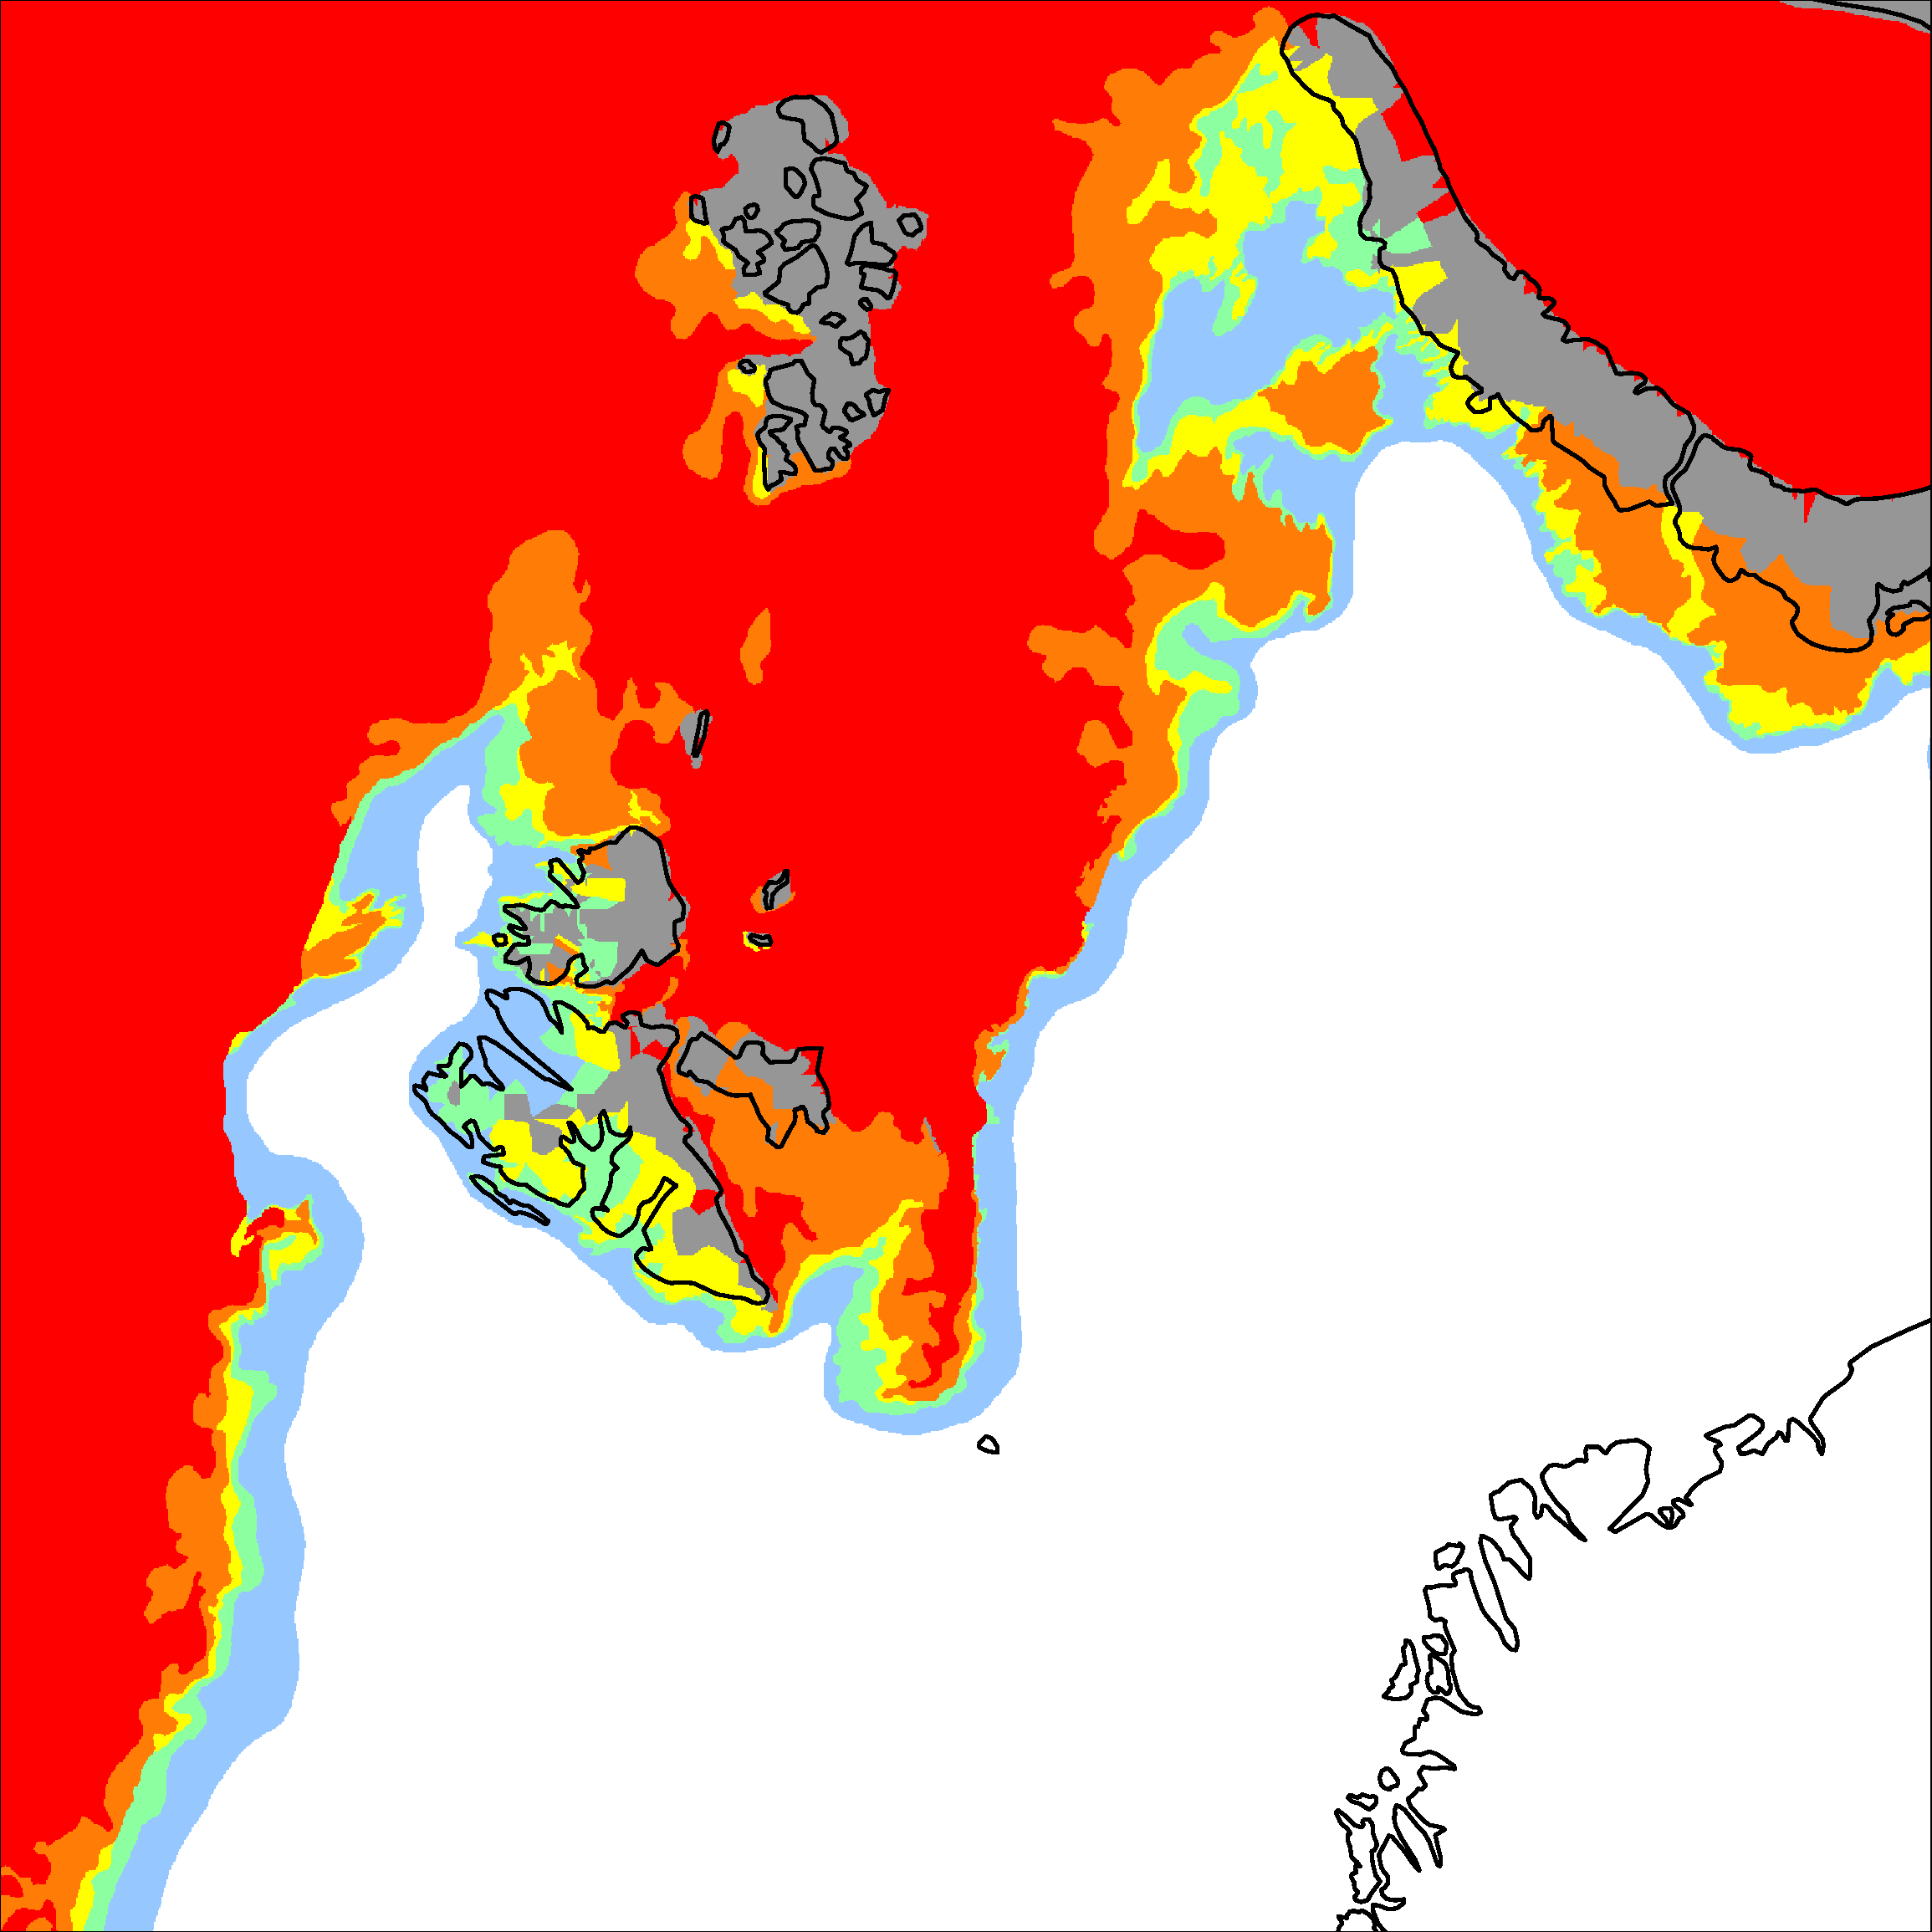
\includegraphics[width=.25\textwidth]{sic.png}};
    \node [above = 0.15cm of sic] (sic_name) {\large Recent Ice Chart};
    % \node [above] at (-6.5,.5) {b)};
    \node[right = 0.25cm of sic_name, align=center] (osi_name) {\large OSI-SAF SIC trend from \\ \large 5 previous days};
    \node (osi) at (sic -| osi_name) {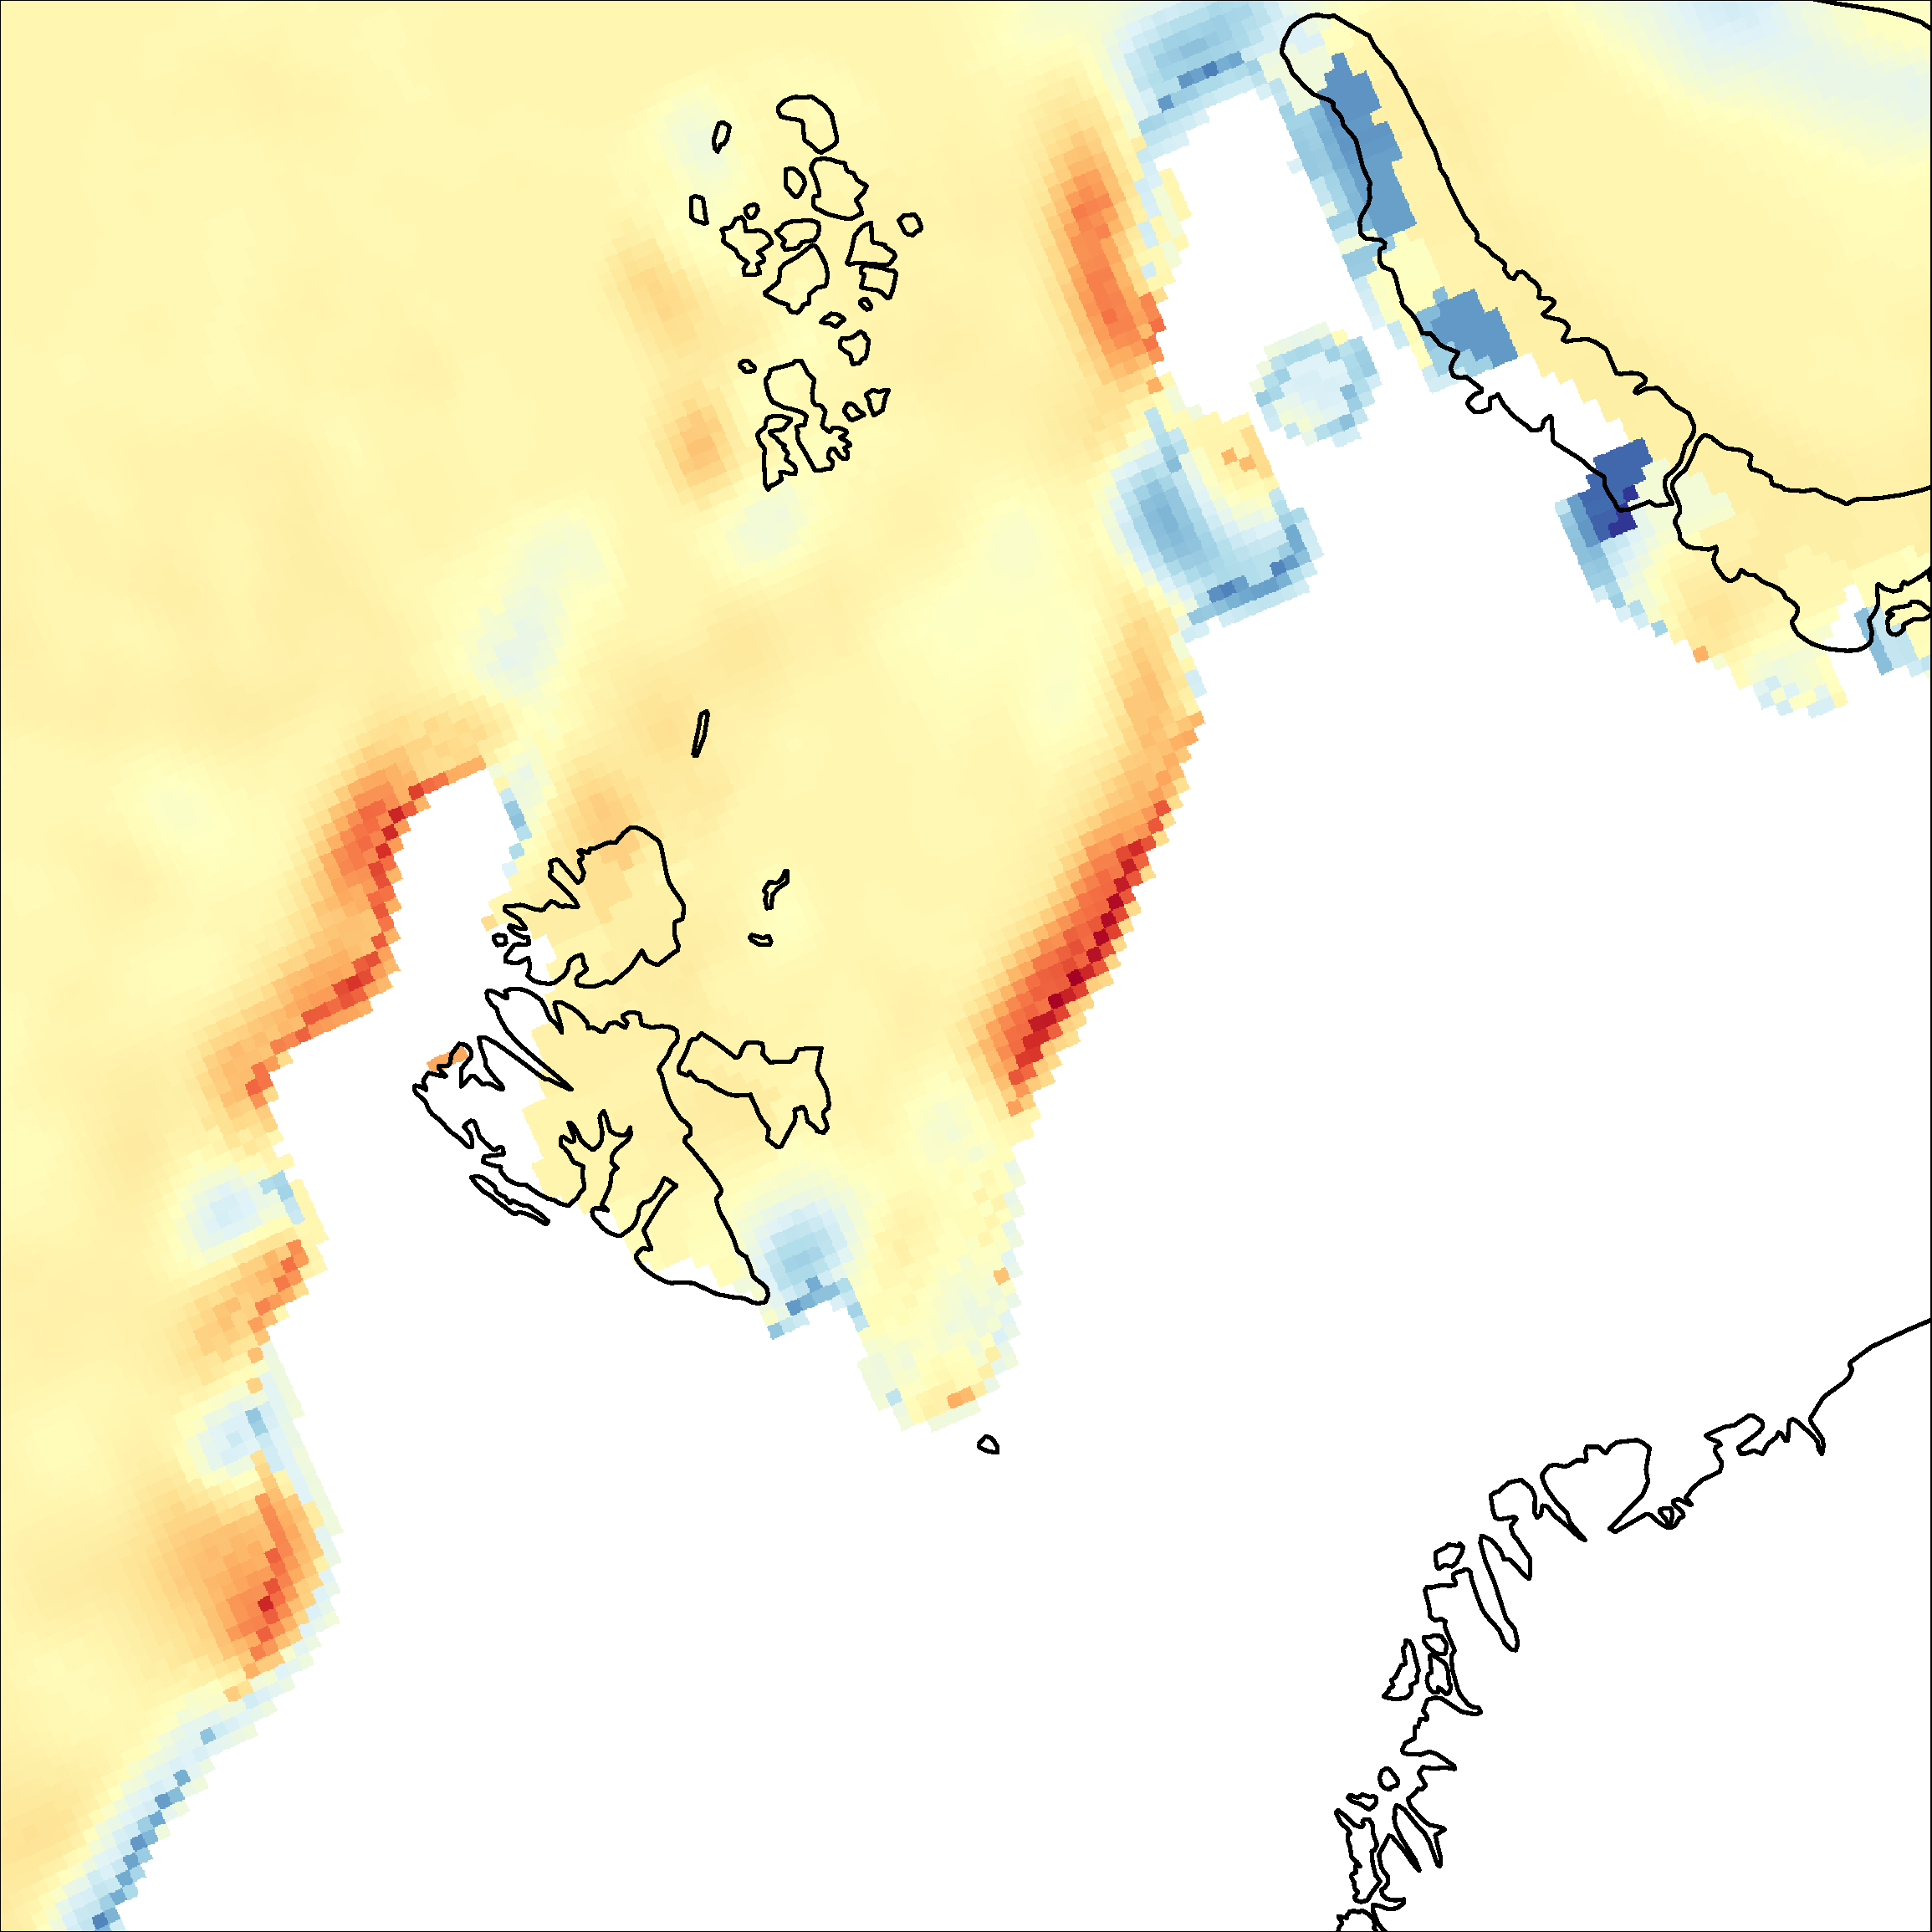
\includegraphics[width=.25\textwidth]{sic_trend.png}};
    % \node [above] at (-6.5,-1.4) {c)};
    \node[right = 0.25cm of osi_name, align = center] (arome_name) {\large AROME Arctic \\ \large t2m and wind forecasts};
    
    \node (aa_forecasts) at (sic -| arome_name) {\includegraphics[width=.25\textwidth]{arome_forecasts.png}};
  
    \node[right = 0.25cm of arome_name, align = center] (mask_name) {\large Land-Sea Mask};
    \node (aa_mask) at (sic -| mask_name) {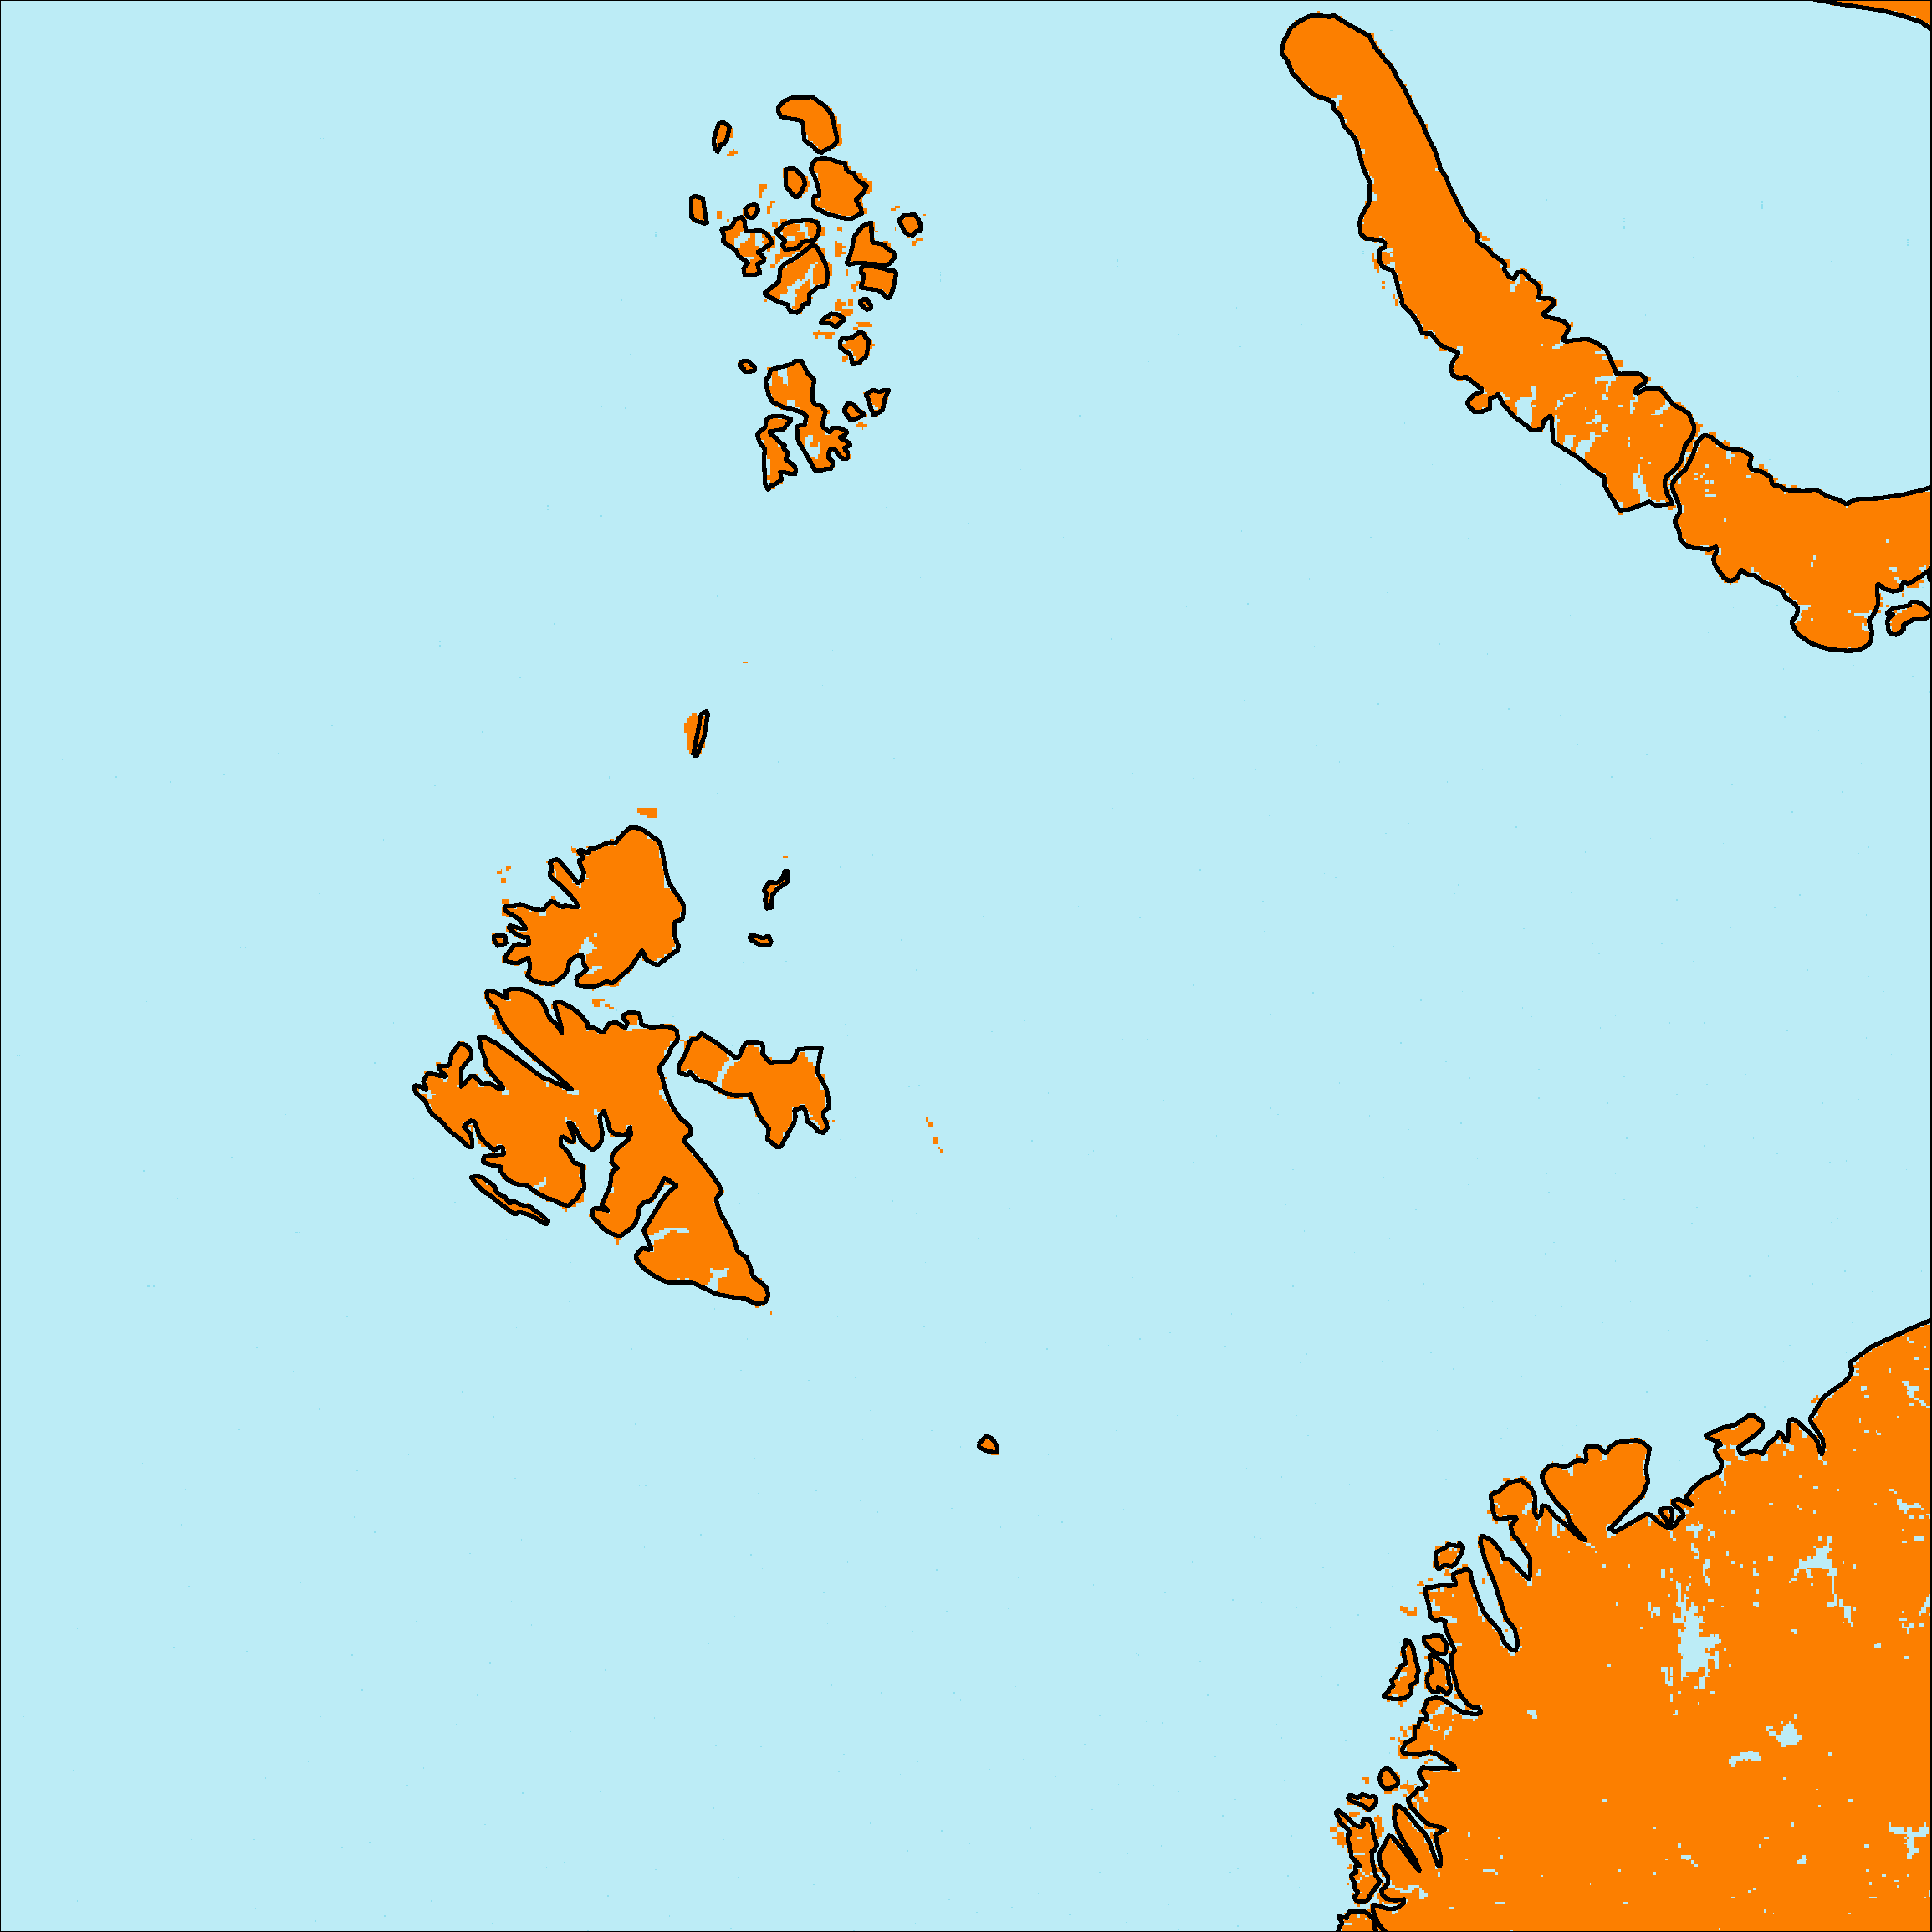
\includegraphics[width=.25\textwidth]{lsmask.png}};
    % \node[draw,single arrow, black,fill=black!30] at (-1.25,0.5,0) {INPUT};
    
    \coordinate[yshift=-5cm] (sample_stack) at ($(osi)!0.5!(aa_forecasts)$);
    \draw [line width=0.8mm, -{Stealth[length=8mm, round]}, shorten >=1.75cm, shorten <=0.2cm]
            (sic.south) -- (sample_stack);
  
    \draw [line width=0.8mm, -{Stealth[length=8mm, round]}, shorten >=1.8cm, shorten <= 0.1cm]
            (osi.south) -- (sample_stack);
  
    \draw [line width=0.8mm, -{Stealth[length=8mm, round]}, shorten >=1.8cm, shorten <= 0.1cm]
            (aa_forecasts.south) -- (sample_stack);
    
    \draw [line width=0.8mm, -{Stealth[length=8mm, round]}, shorten >=2cm, shorten <=0.2cm]
            (aa_mask.south) -- (sample_stack);
  
    \node at (sample_stack) (stack1) {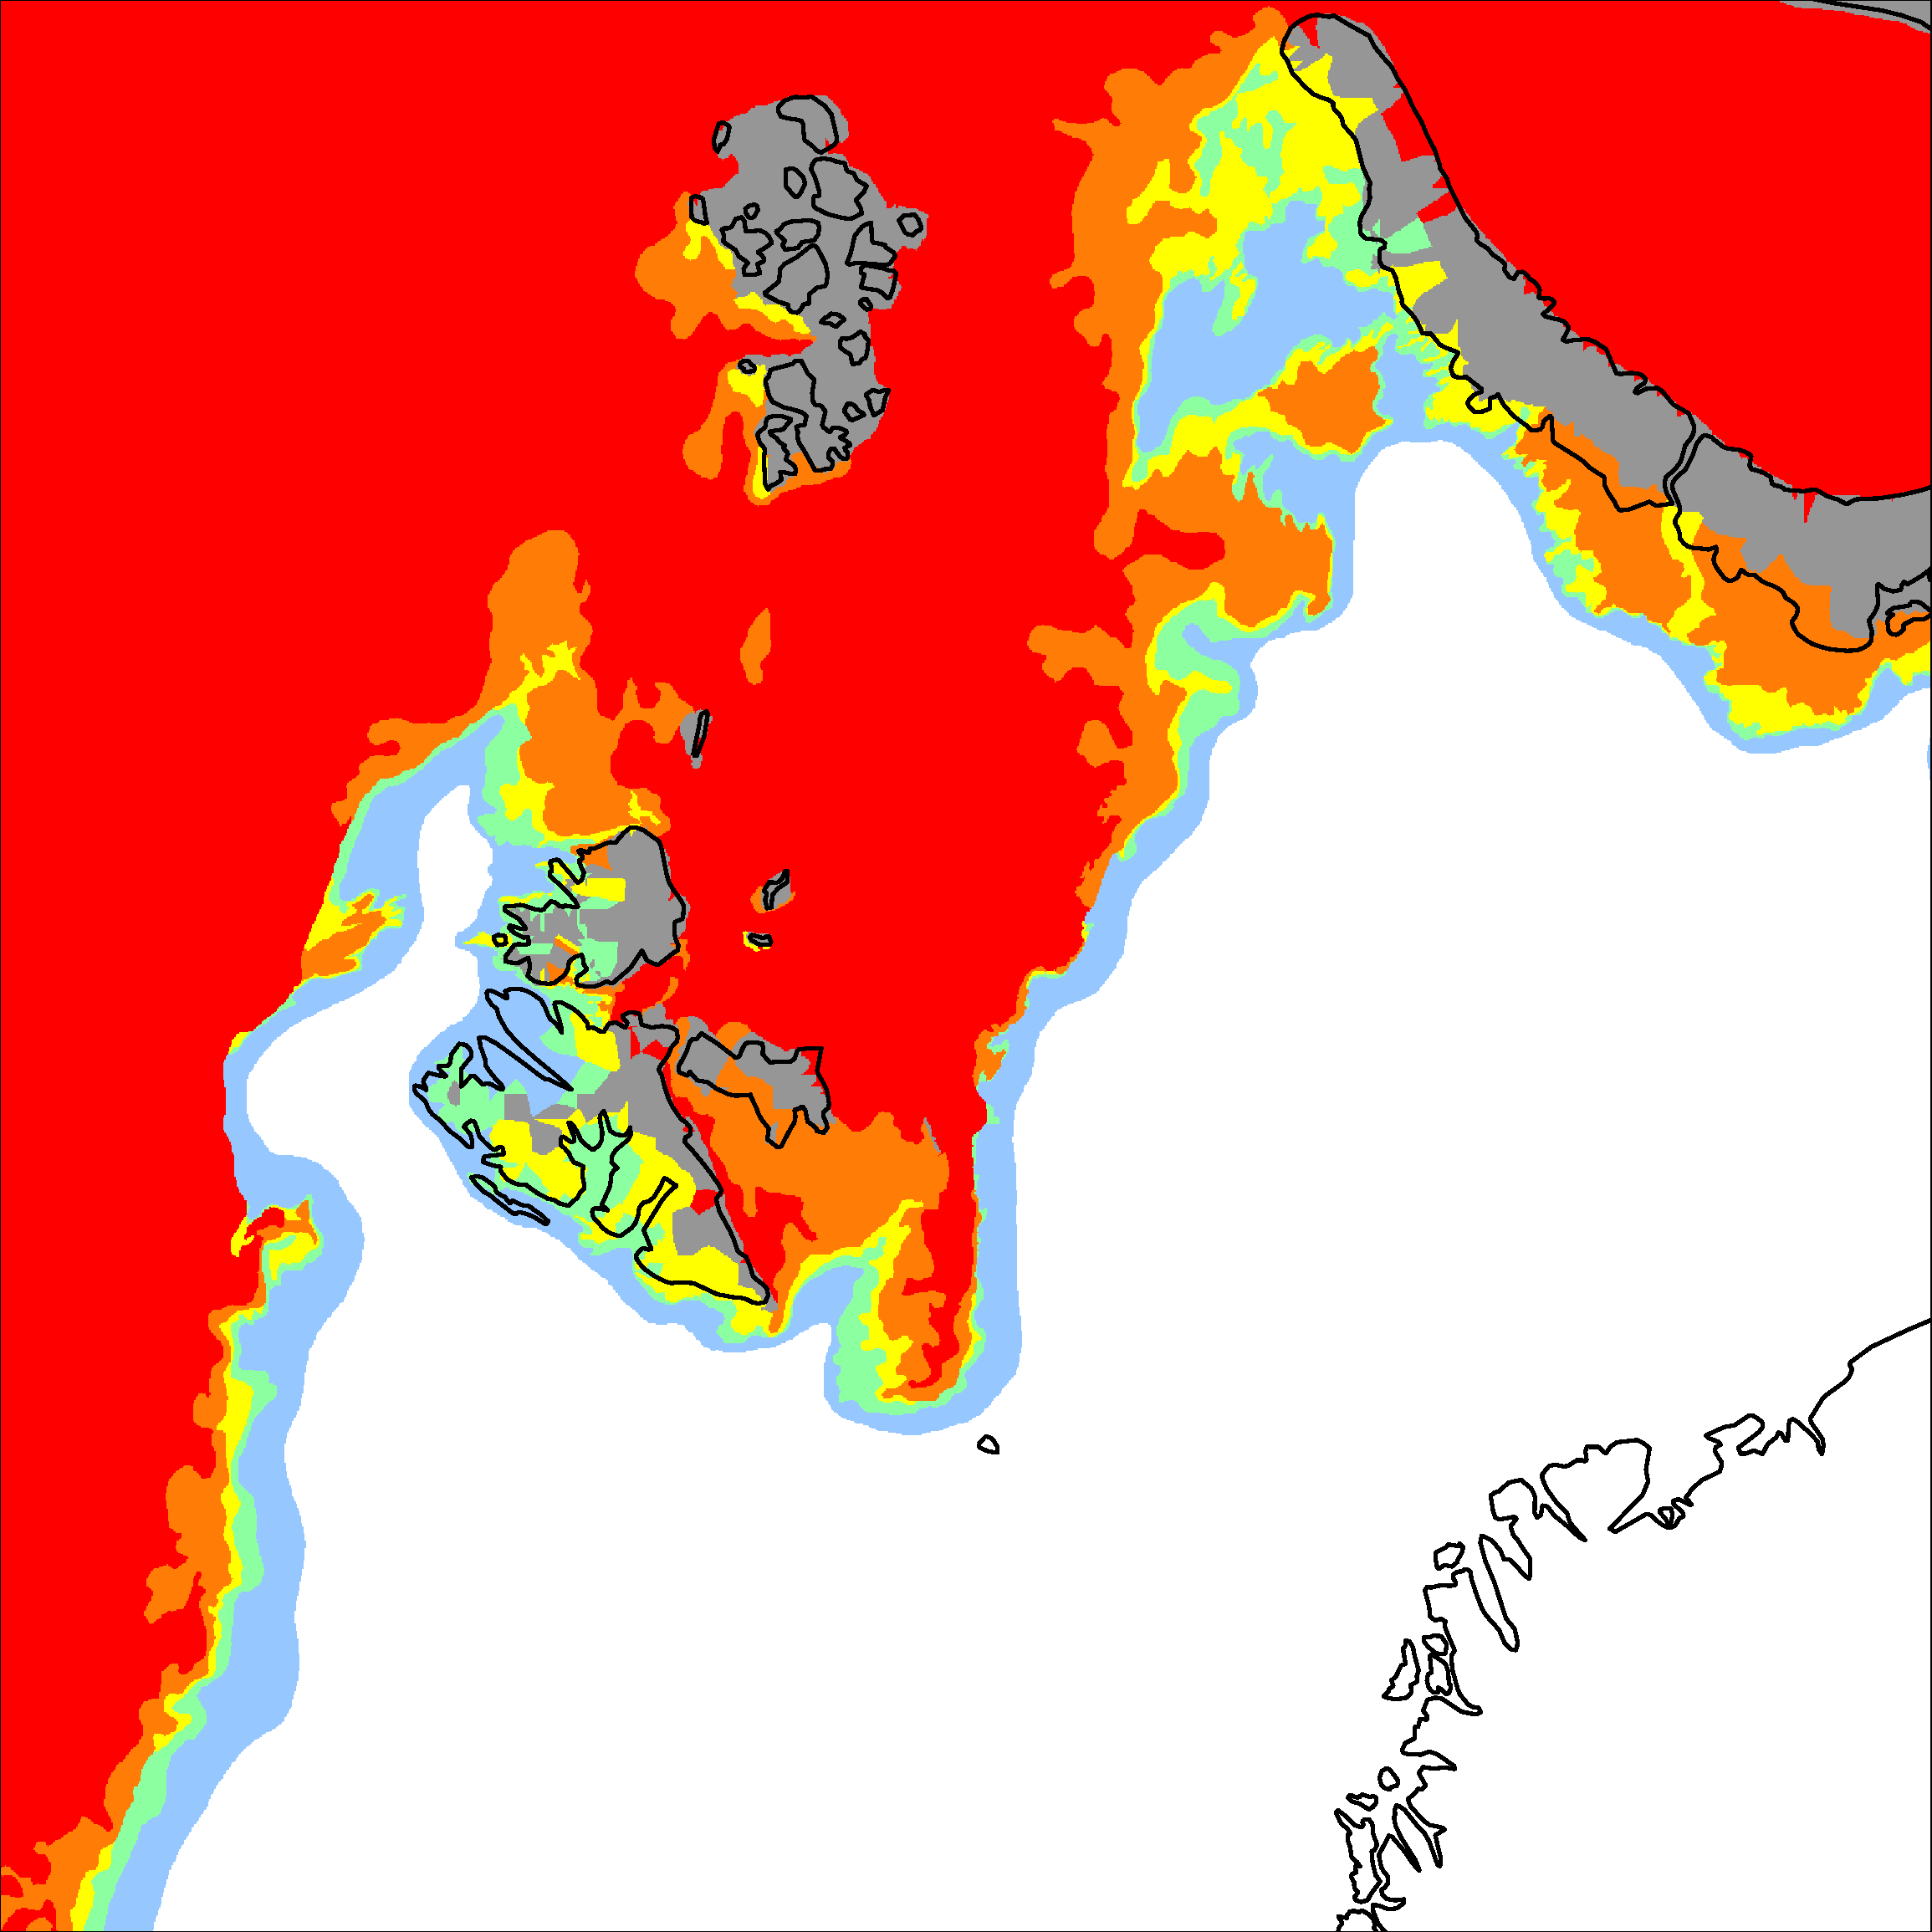
\includegraphics[width=.15\textwidth]{sic.png}};
    \node[yshift = -0.1cm, xshift = 0.1cm] at (sample_stack) (stack2) {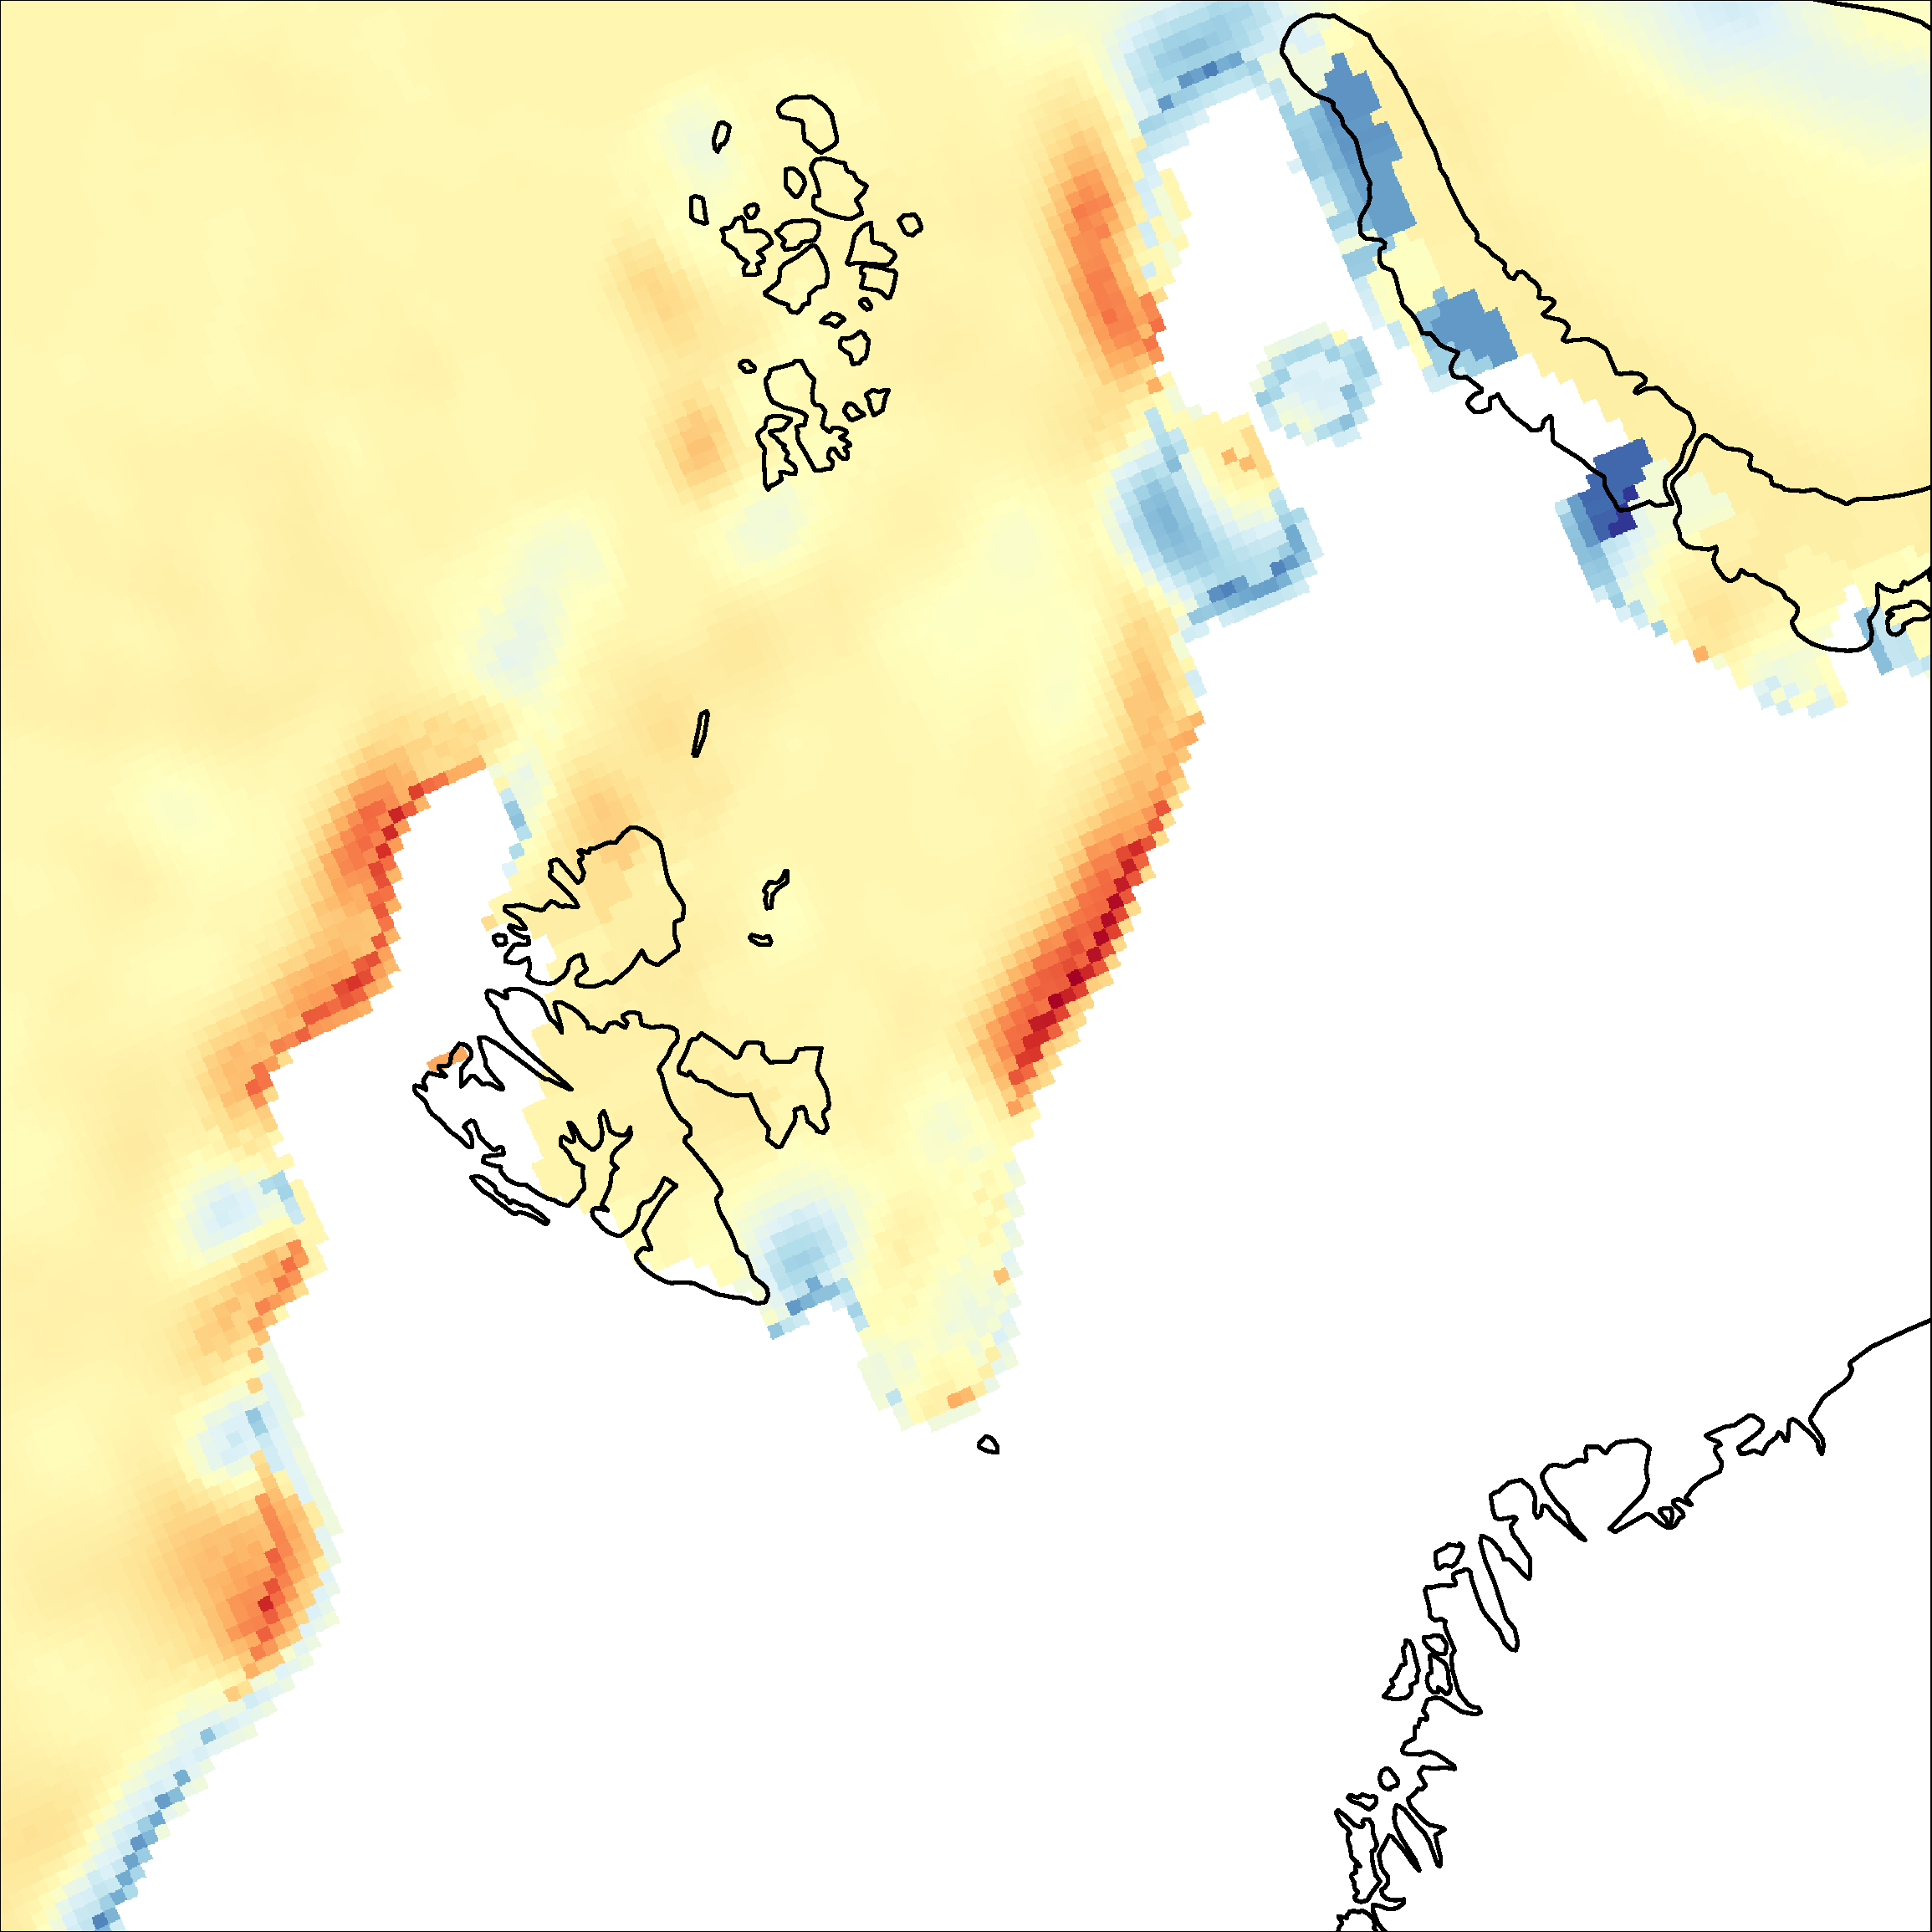
\includegraphics[width=.15\textwidth]{sic_trend.png}};
    \node[yshift = -0.2cm, xshift = 0.2cm] at (sample_stack) (stack3) {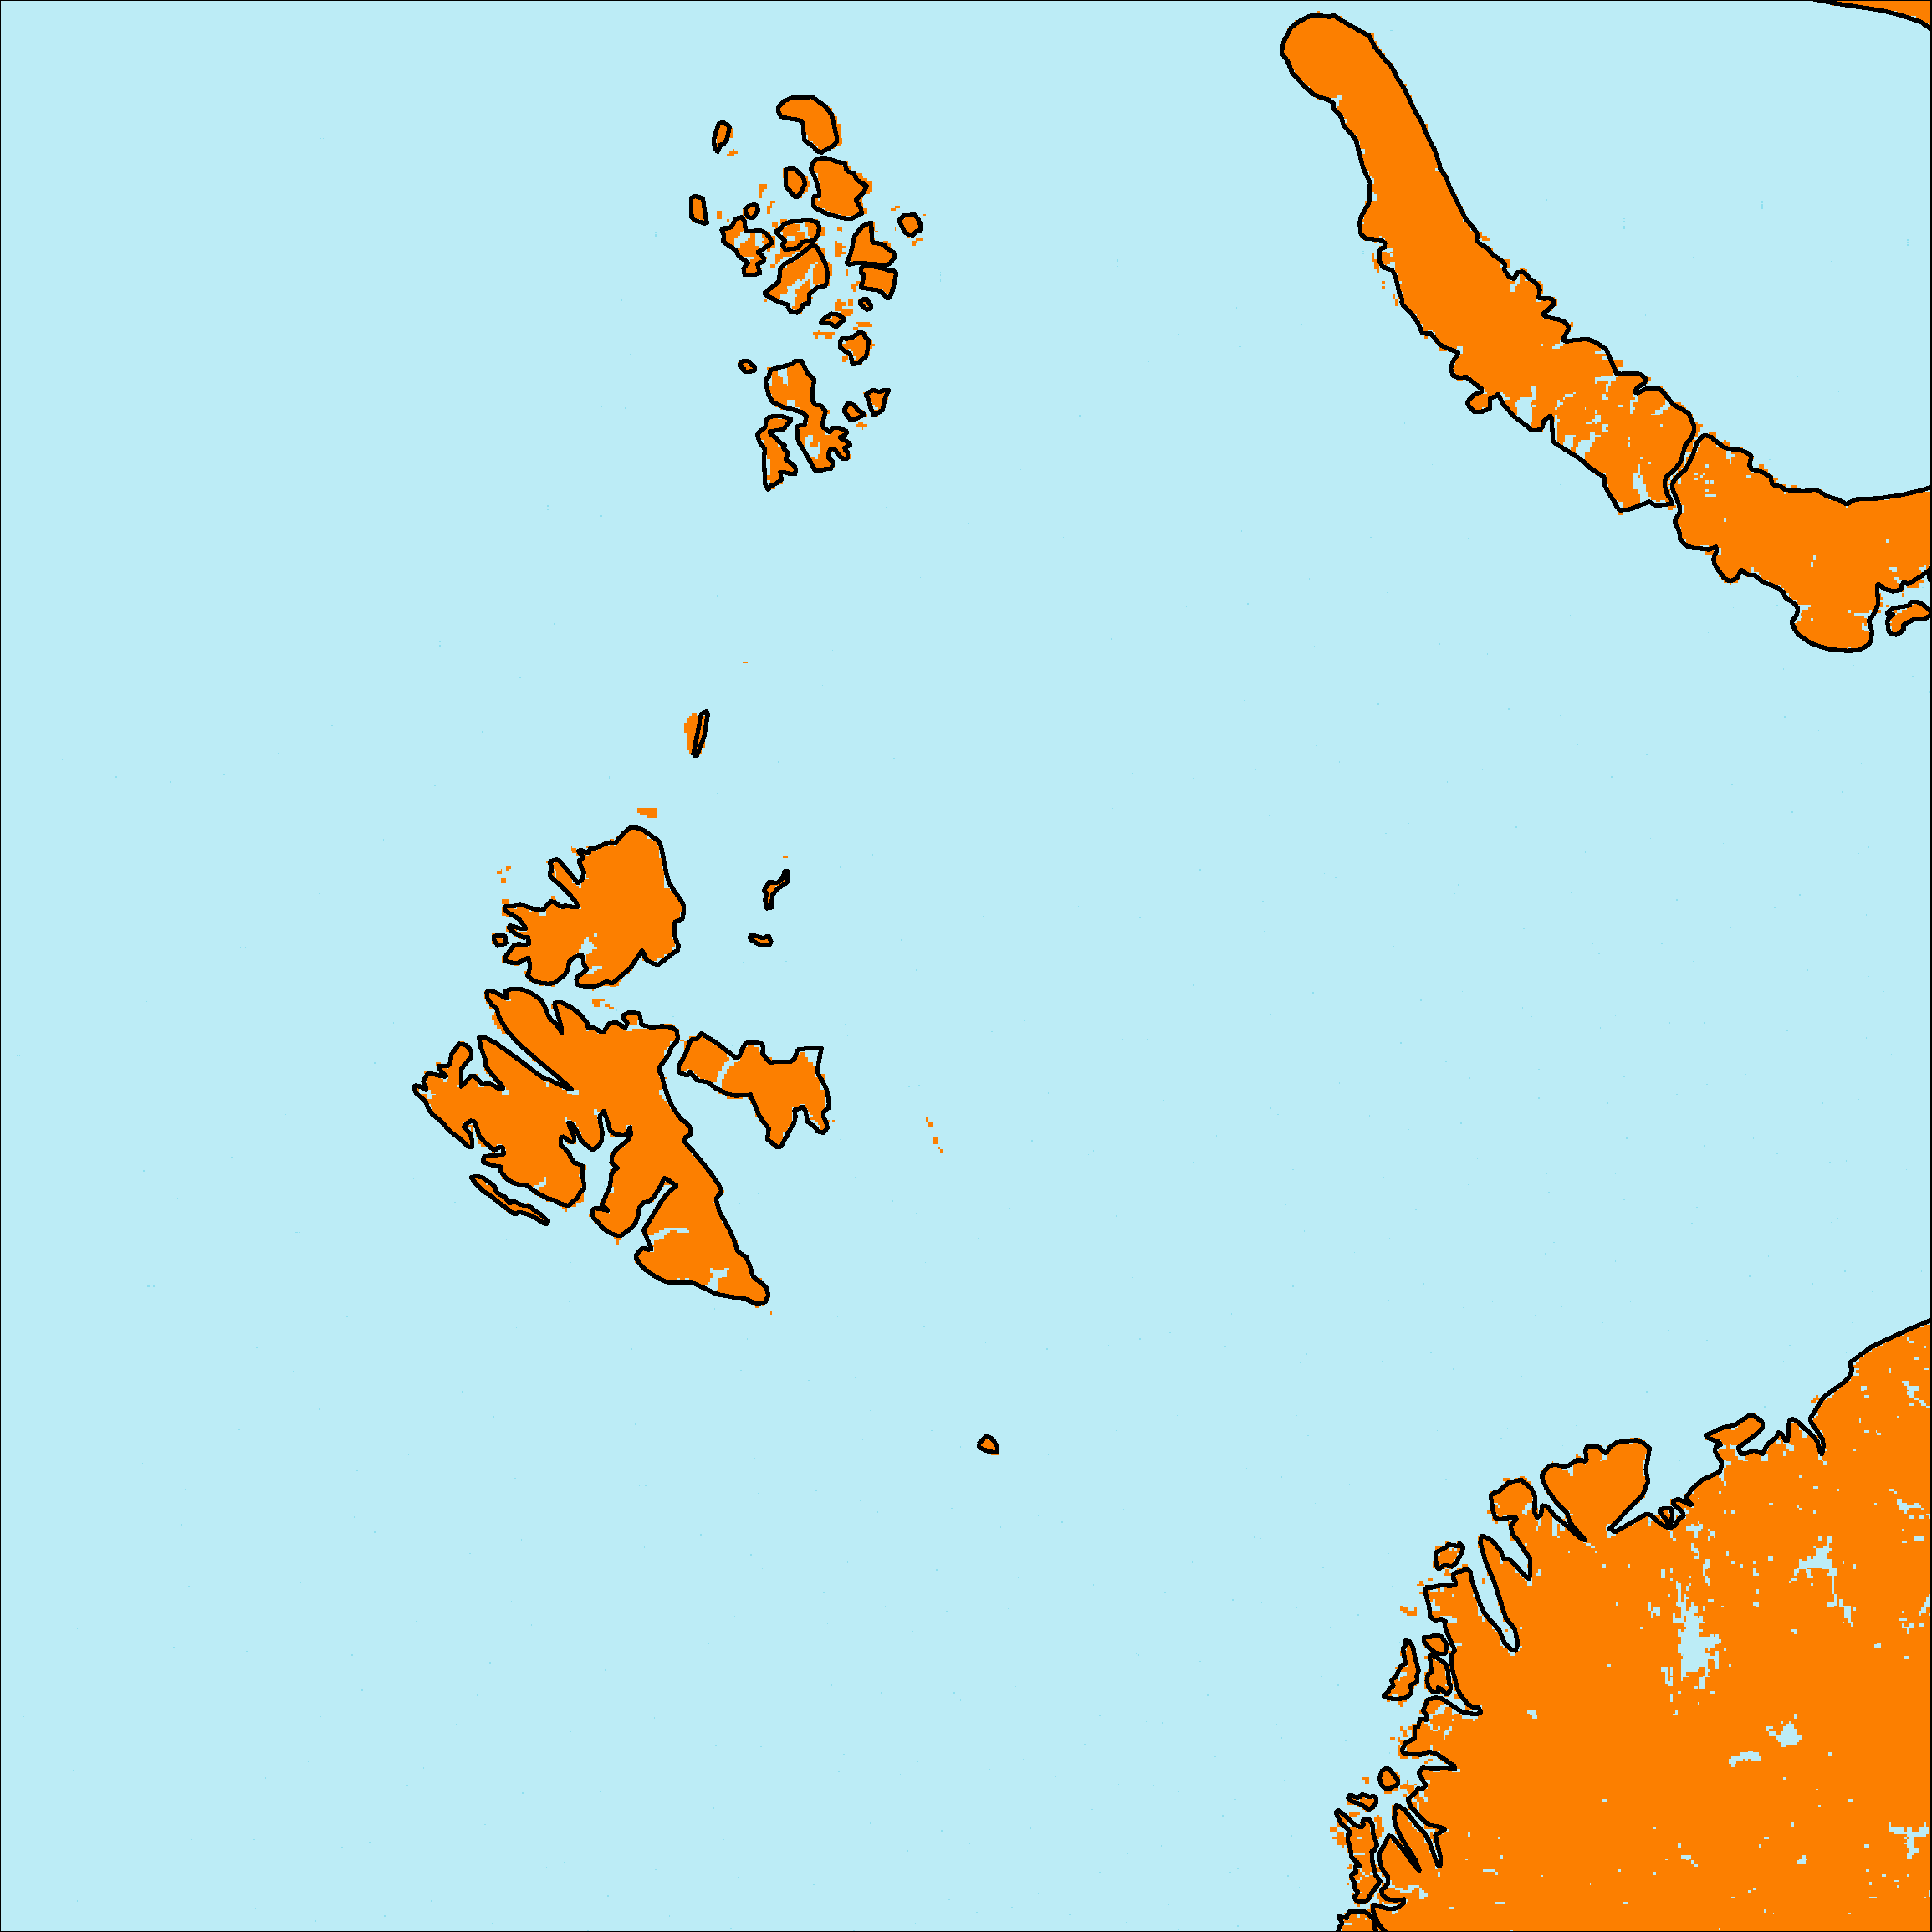
\includegraphics[width=.15\textwidth]{lsmask.png}};
    \node[yshift = -0.3cm, xshift = 0.3cm] at (sample_stack) (stack4) {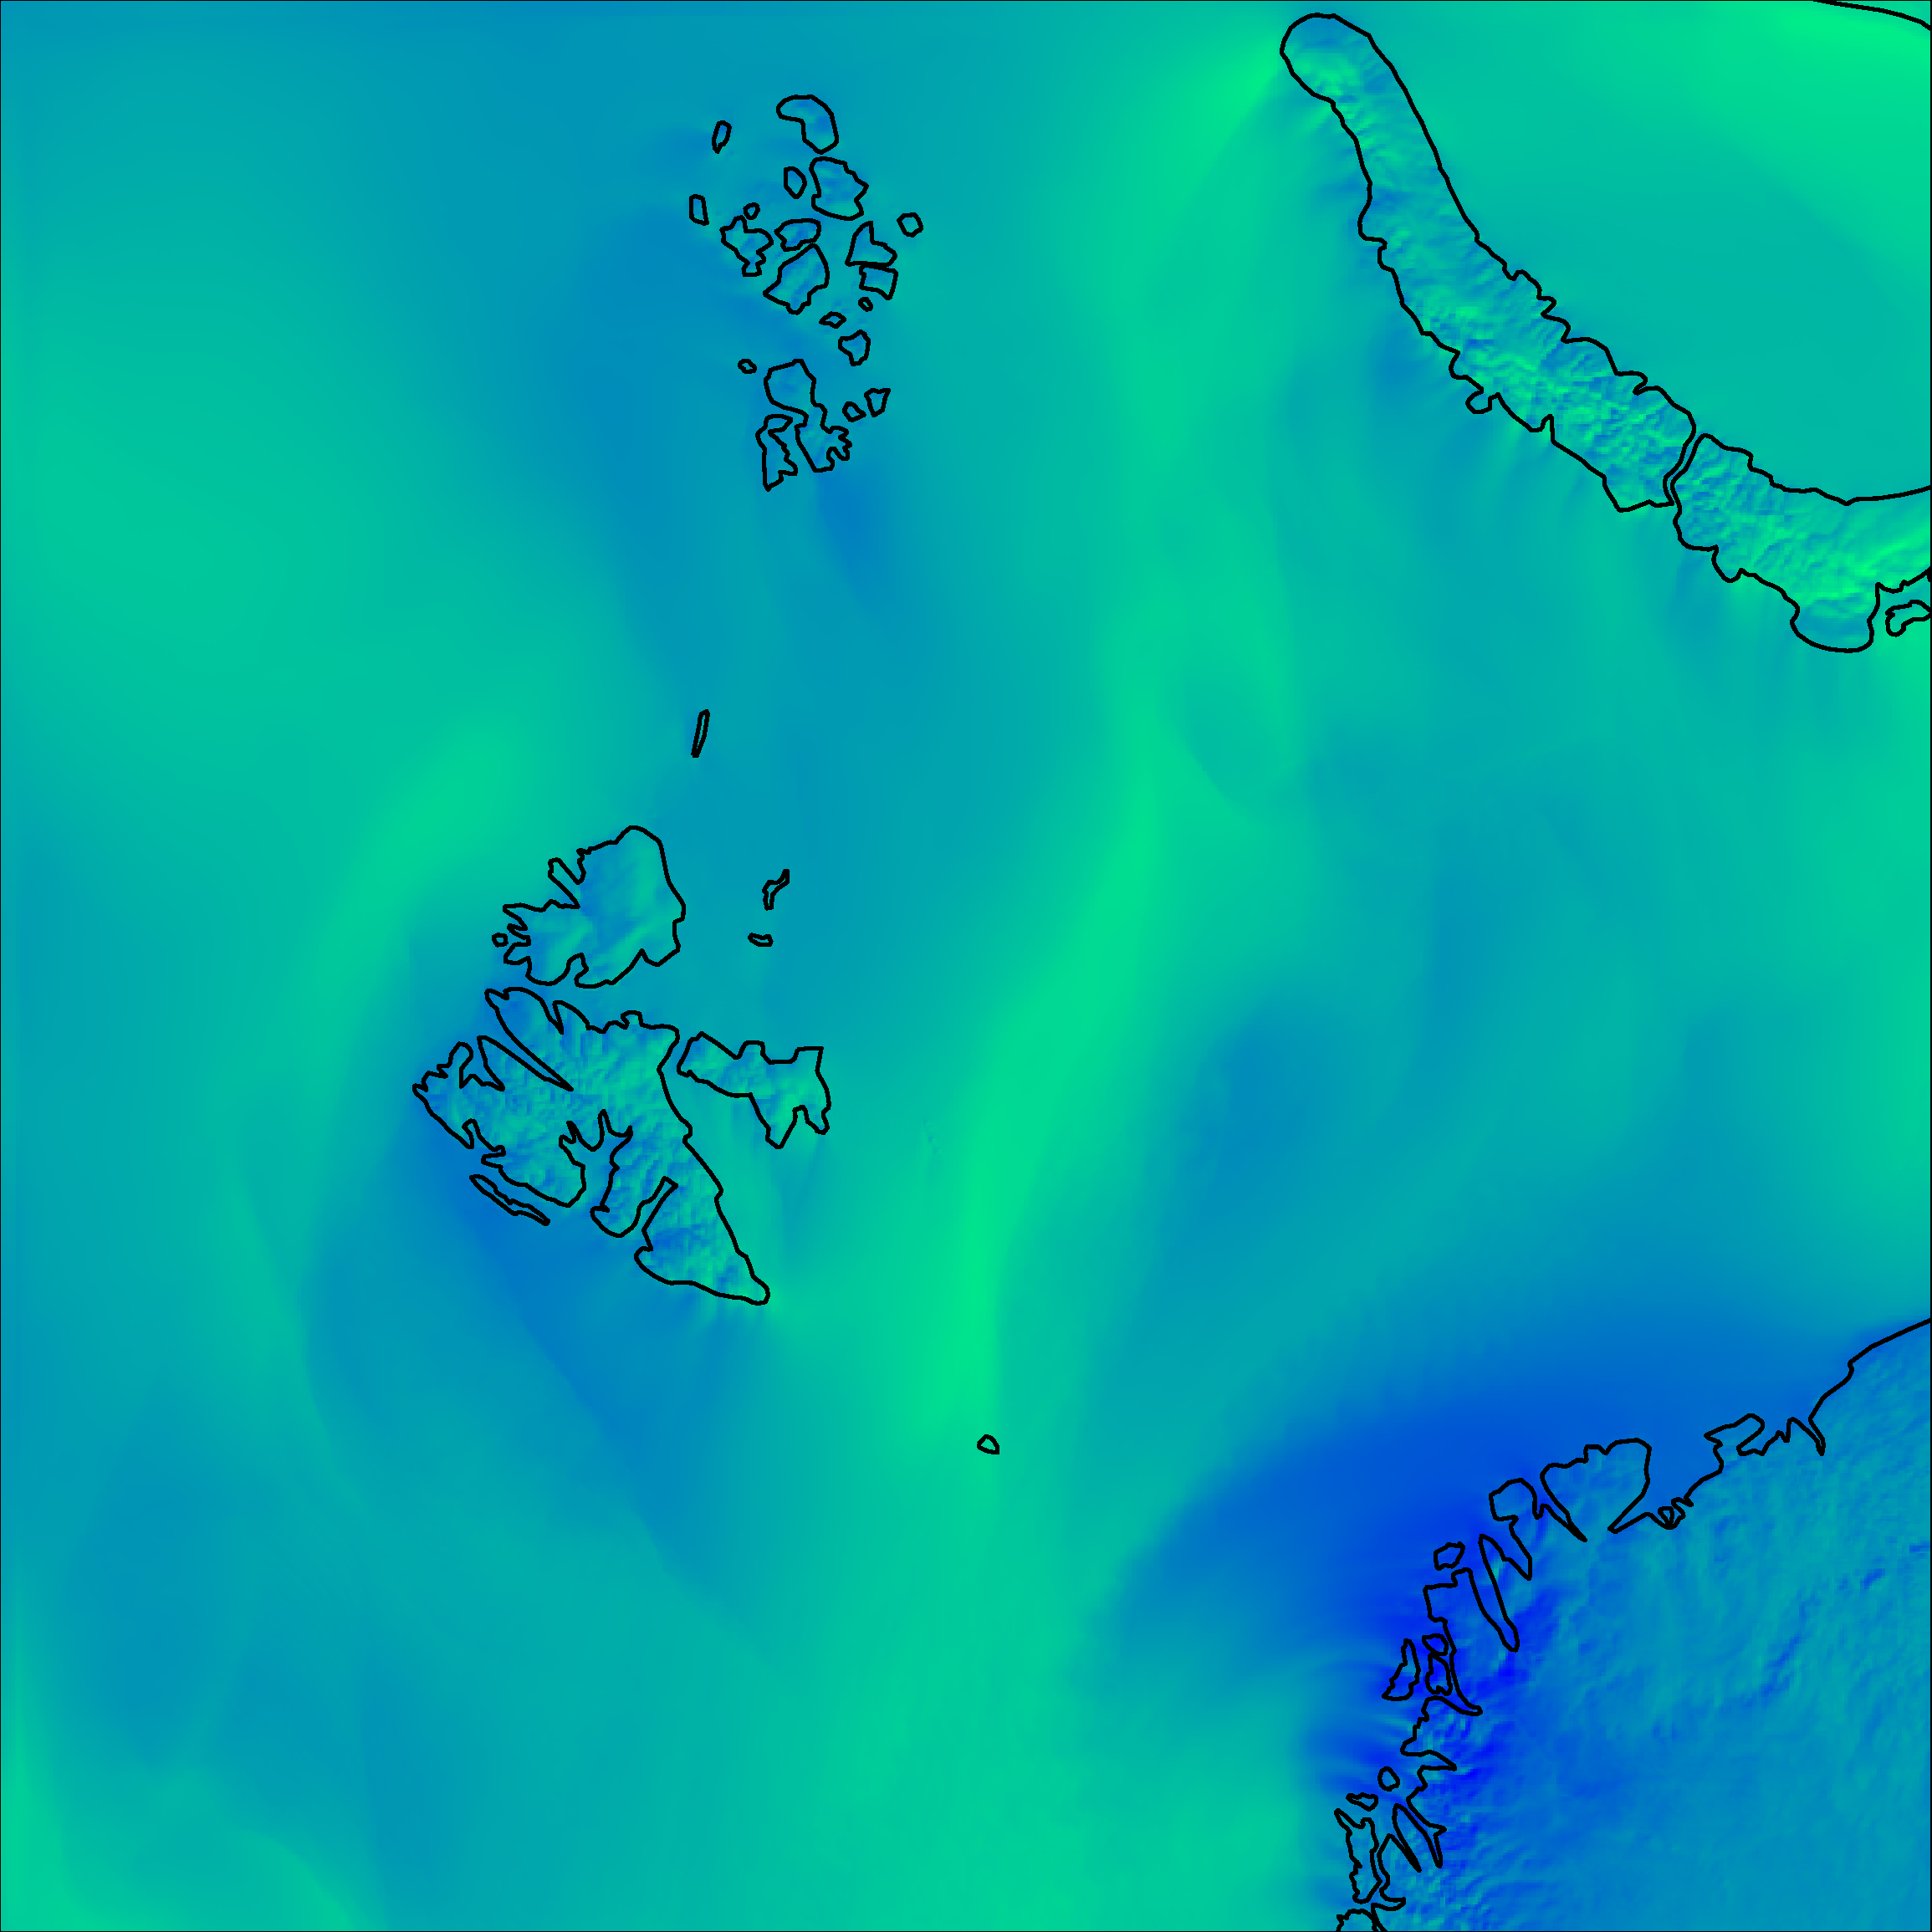
\includegraphics[width=.15\textwidth]{xwind.png}};
    \node[yshift = -0.4cm, xshift = 0.4cm] at (sample_stack) (stack5) {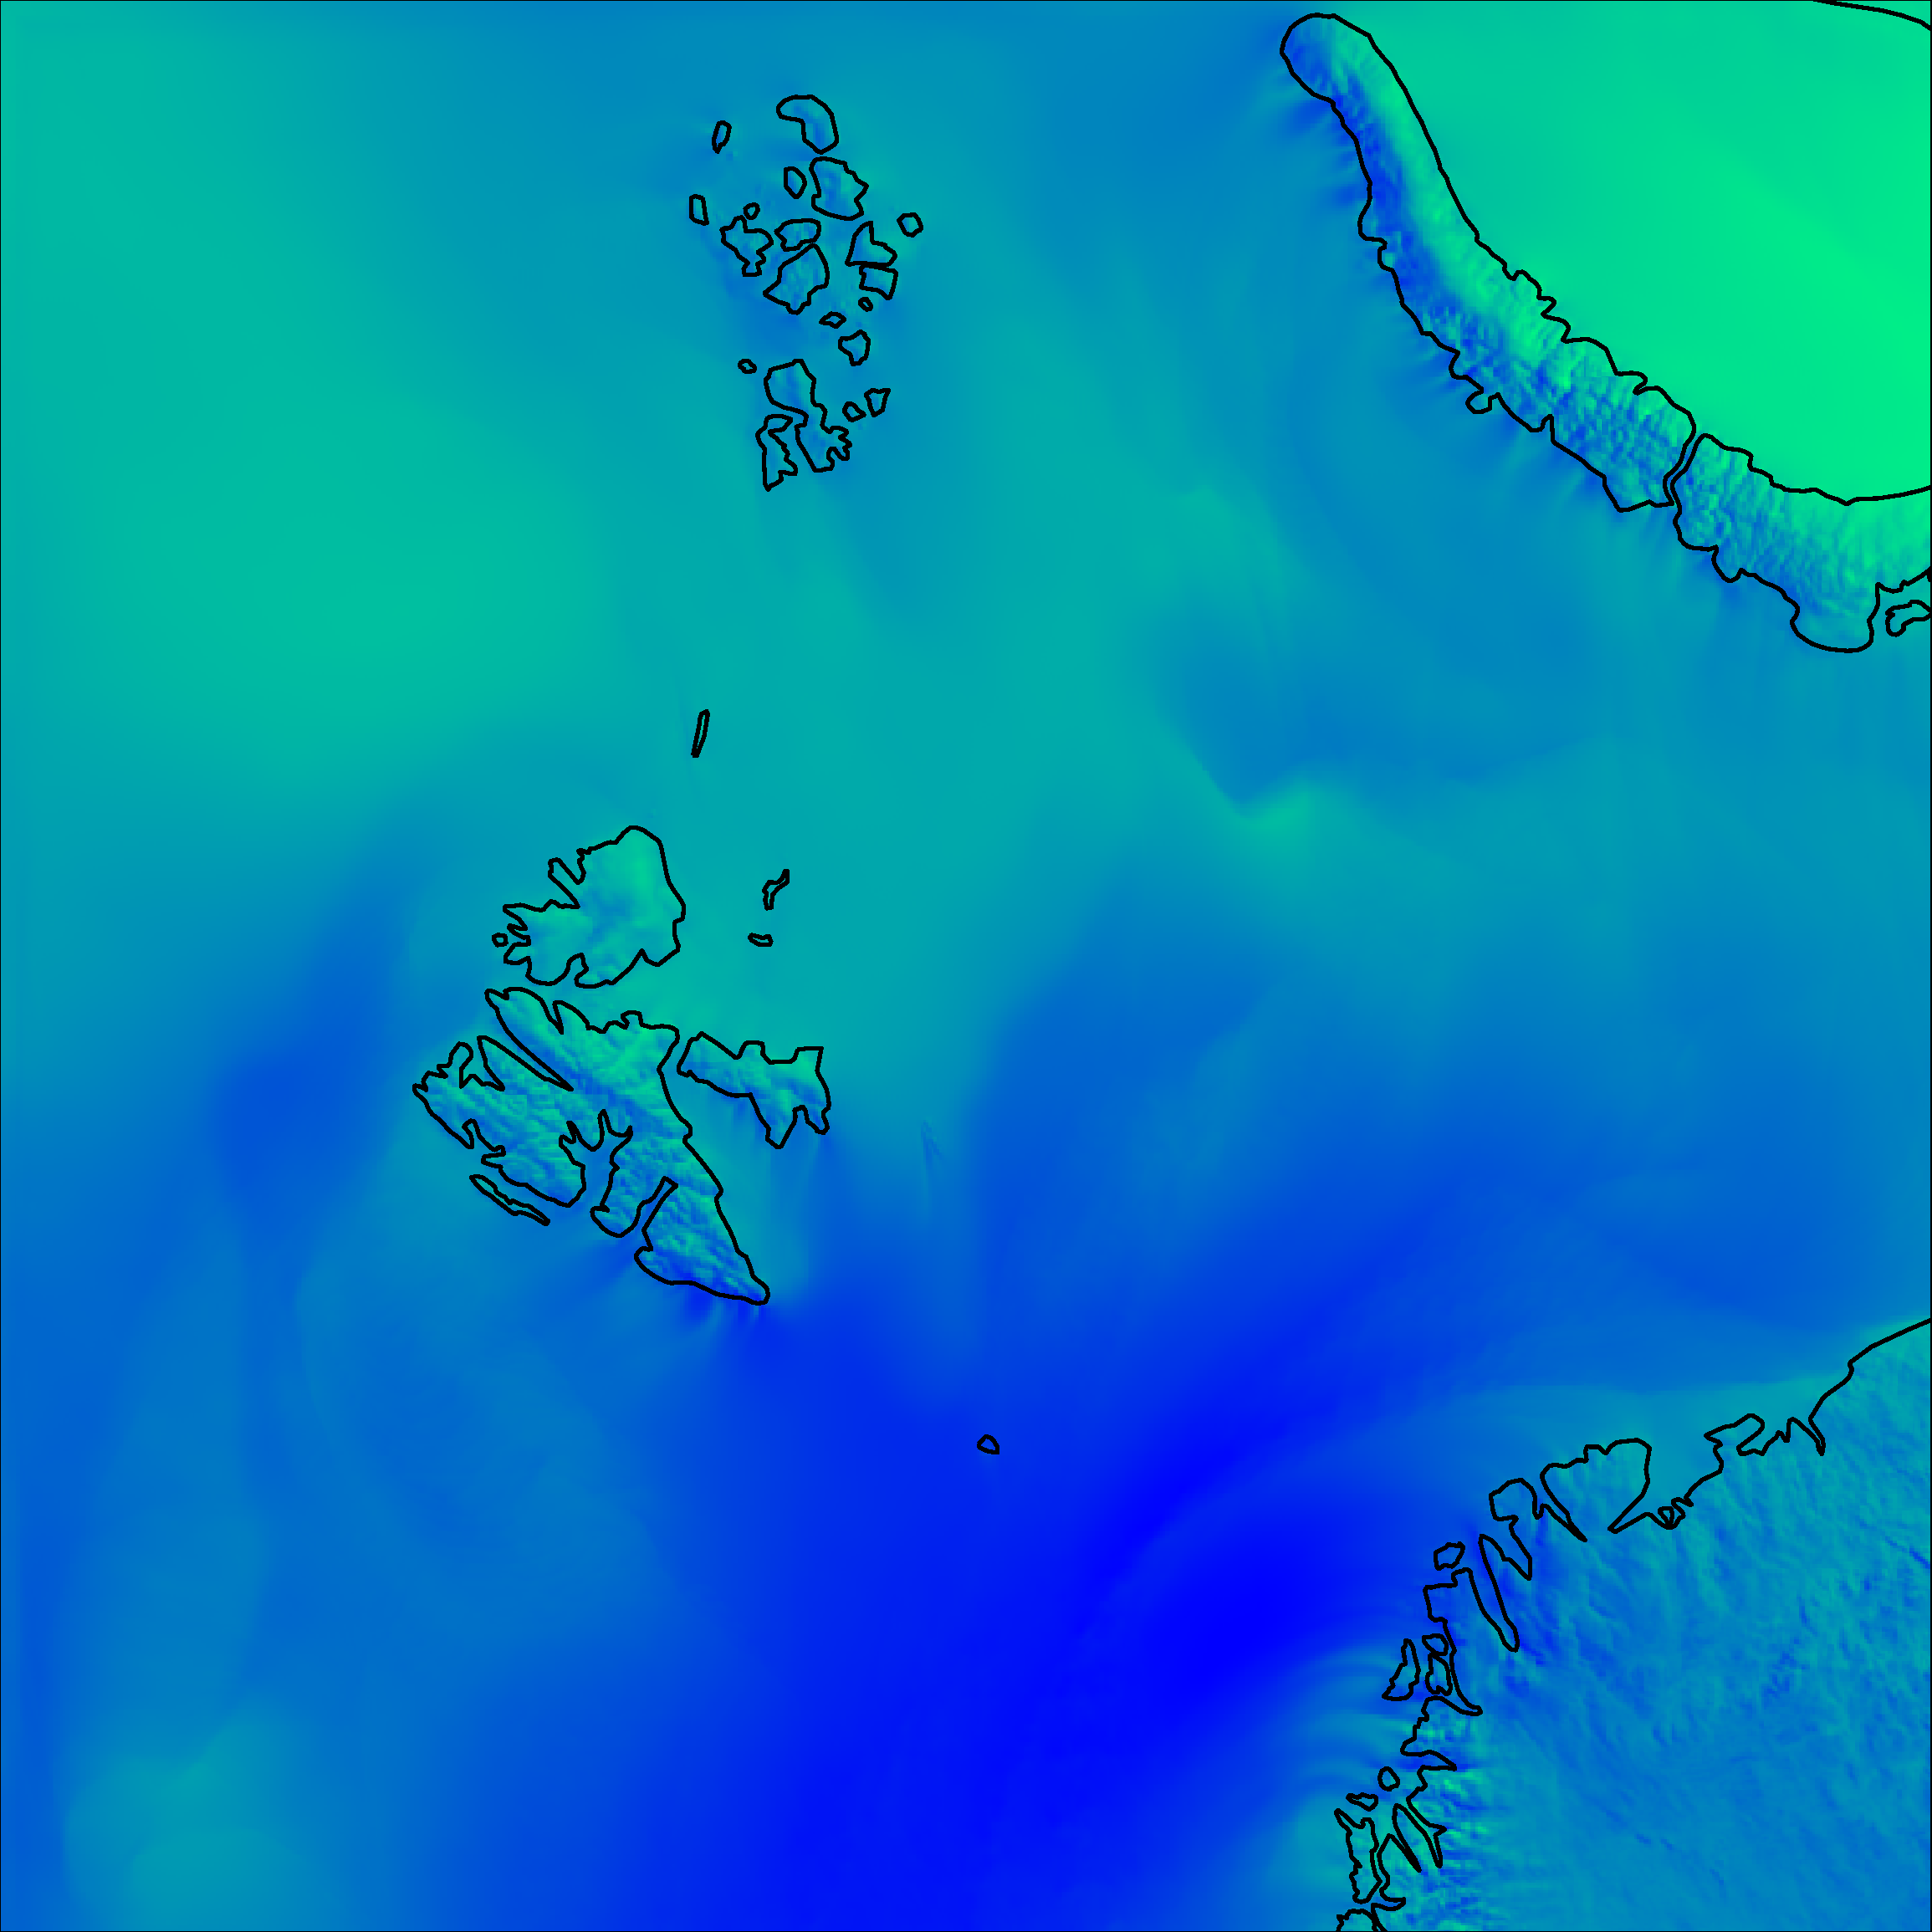
\includegraphics[width=.15\textwidth]{ywind.png}};
    \node[yshift = -0.5cm, xshift = 0.5cm] at (sample_stack) (stack6) {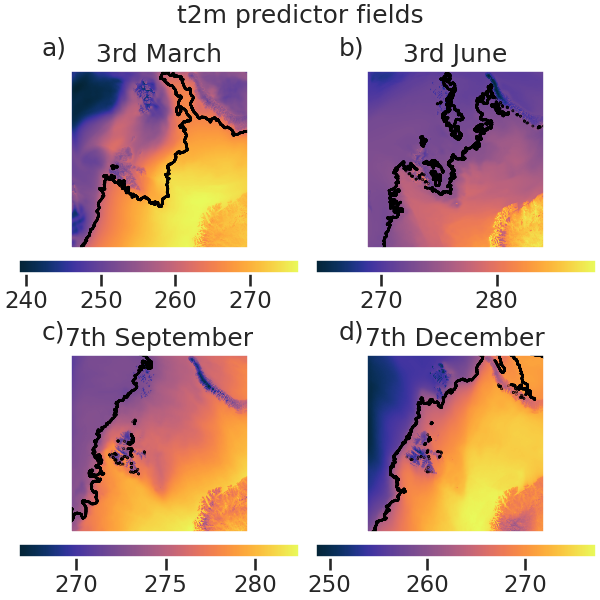
\includegraphics[width=.15\textwidth]{t2m.png}};
    
    \node[left = 1.3cm of sample_stack] (stack_name) {\large Sample};
  
    \node[below = 4cm of sample_stack, rectangle, draw=orange!50, fill=orange!20, thick, minimum width = 2cm, minimum height = 2cm, align = center] (unet) {U-NET};
   
    
    \draw [line width=0.8mm, -{Stealth[length=8mm, round]}, shorten >= 0.1cm, shorten <= 1.8cm] (sample_stack.south) -- (unet) node[midway, fill = white, anchor = center, text = black, yshift = -0.5cm] {\large Predictor variables};
  
    \node (sic_target) at (unet -| sic) {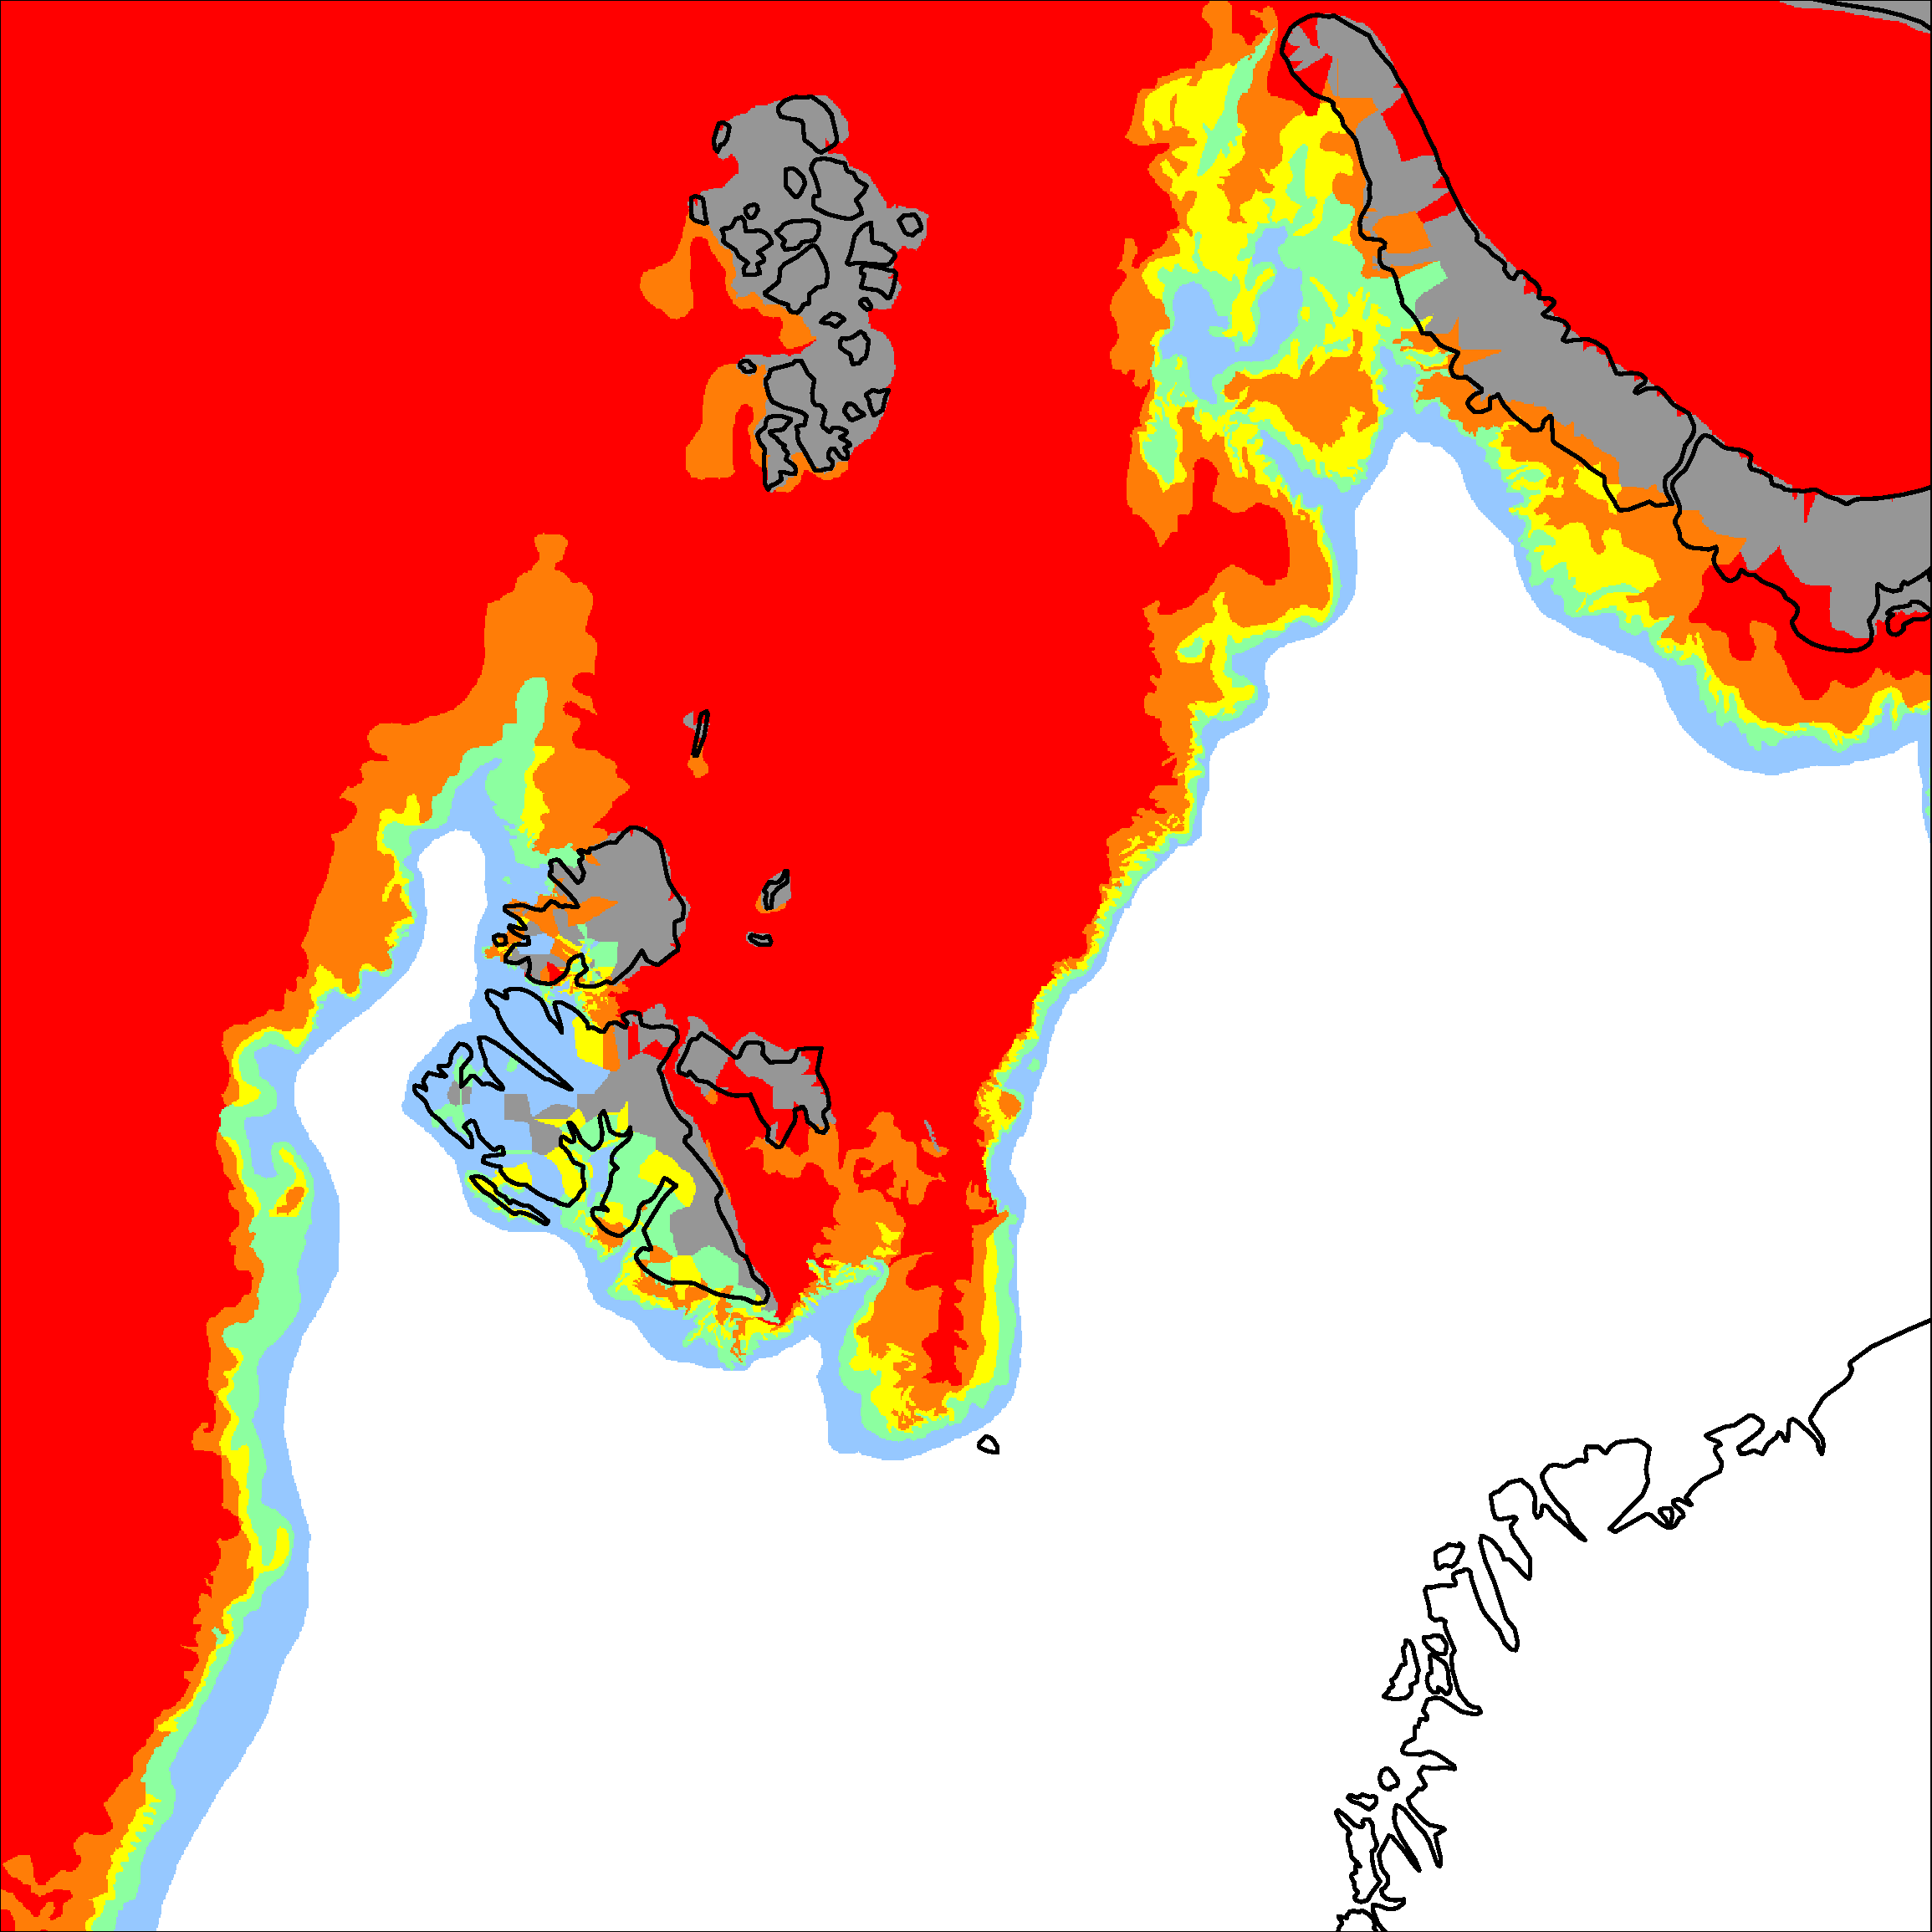
\includegraphics[width=.25\textwidth]{sic_target.png}};
    \node [above = 0cm of sic_target] (sic_target_name) {\large Target Ice Chart};
    \draw [line width=0.8mm, -{Stealth[length=8mm, round]}, shorten >= 0.1cm, shorten <= 0.1cm] (sic_target.east) -- node [midway, above = 0.2cm, xshift = -0.2cm] {\large Target variable} (unet.west);
  
    \node [inner ysep=3mm, below = 2cm of unet] (sic_pred) {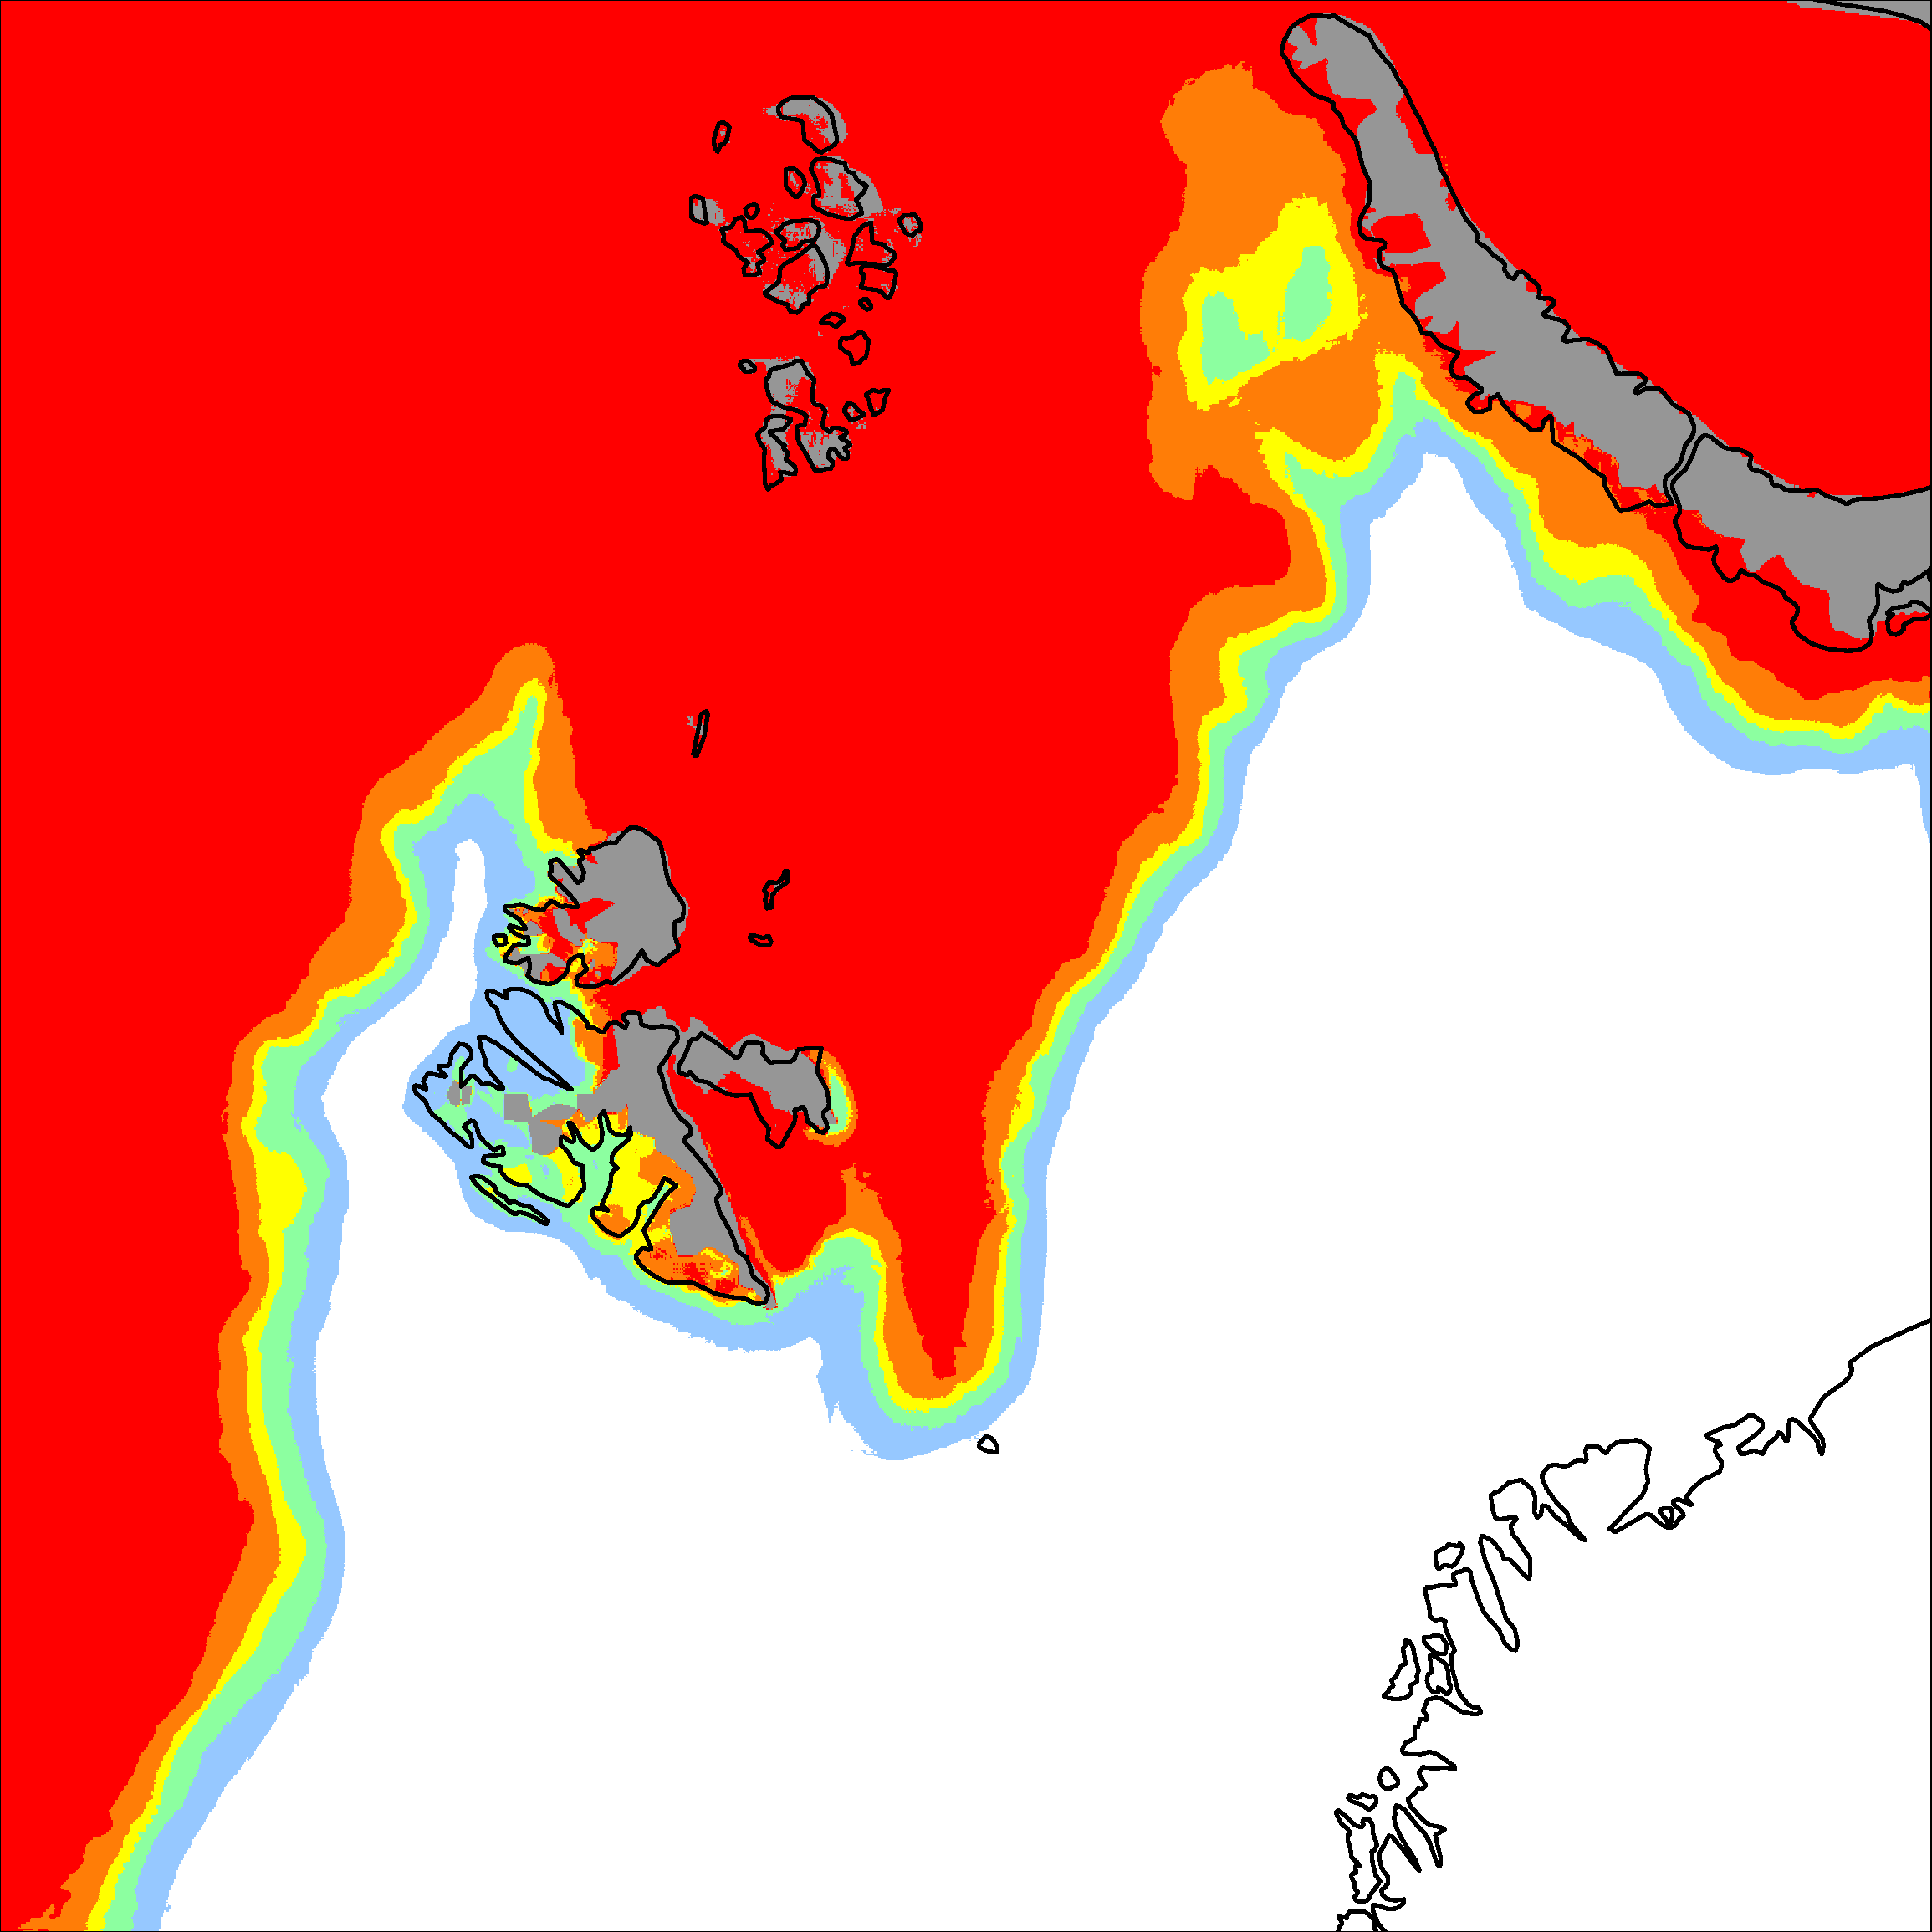
\includegraphics[width=.25\textwidth]{20220105.png}};
    \node [above = 0cm of sic_pred] (sic_pred_name) {\large Predicted Ice Chart};
    \draw [line width=0.8mm, -{Stealth[length=8mm, round]}, shorten >= 0.1cm, shorten <= 0.1cm] (unet.south) -- (sic_pred_name.north);
  
      
\end{tikzpicture}

\end{document}